\documentclass[12pt,a4paper]{report}
\usepackage[pdftex]{graphicx}
\usepackage{url} 
\usepackage[bookmarks, colorlinks=false, pdfborder={0 0 0}, pdftitle={Final Report}, pdfauthor={S.Piraveen}, pdfsubject={Industrial Training Report}, pdfkeywords={cs3992}]{hyperref} 
\usepackage{lipsum}% for auto generating text
\usepackage{afterpage}
\usepackage{xcolor}
\usepackage{fontawesome5}
\usepackage{hyperref}
\usepackage{wrapfig}
\usepackage{titlesec}
\usepackage{float}
\usepackage{subcaption}
\graphicspath{ {figures/} }
\usepackage[printonlyused,withpage]{acronym}
\usepackage{array}
\usepackage{biblatex}
\addbibresource{FinalReport.bib}

\DeclareFontFamily{U}{fontawesomeOne}{}
\DeclareFontShape{U}{fontawesomeOne}{m}{n}
 {<-> FontAwesome--fontawesomeone}{}
\DeclareRobustCommand\FAone{\fontencoding{U}\fontfamily{fontawesomeOne}\selectfont} 

\begin{document}

\titleclass{\subsubsubsection}{straight}[\subsection]

\newcounter{subsubsubsection}[subsubsection]
\renewcommand\thesubsubsubsection{\thesubsubsection.\arabic{subsubsubsection}}
\renewcommand\theparagraph{\thesubsubsubsection.\arabic{paragraph}} % optional; useful if paragraphs are to be numbered

\titleformat{\subsubsubsection}
 {\normalfont\normalsize\bfseries}{\thesubsubsubsection}{1em}{}
\titlespacing*{\subsubsubsection}
{0pt}{3.25ex plus 1ex minus .2ex}{1.5ex plus .2ex}

\makeatletter
\renewcommand\paragraph{\@startsection{paragraph}{5}{\z@}%
 {3.25ex \@plus1ex \@minus.2ex}%
 {-1em}%
 {\normalfont\normalsize\bfseries}}
\renewcommand\subparagraph{\@startsection{subparagraph}{6}{\parindent}%
 {3.25ex \@plus1ex \@minus .2ex}%
 {-1em}%
 {\normalfont\normalsize\bfseries}}
\def\toclevel@subsubsubsection{4}
\def\toclevel@paragraph{5}
\def\toclevel@paragraph{6}
\def\l@subsubsubsection{\@dottedtocline{4}{7em}{4em}}
\def\l@paragraph{\@dottedtocline{5}{10em}{5em}}
\def\l@subparagraph{\@dottedtocline{6}{14em}{6em}}
\makeatother

\setcounter{secnumdepth}{4}
\setcounter{tocdepth}{4}
\renewcommand\bibname{References}


\begin{titlepage}

\begin{center}
% page color is orange
\pagecolor{orange}\afterpage{\nopagecolor}




% Title
\Large \textup{{\bf University of Moratuwa} \\ Faculty of Engineering }\\[0.7in]


        

\includegraphics[width=50mm]{download.png}\\[0.2in]

% Registered Module No : CS3992\\[0.2in]
\textup{Registered Module No: CS3992}\\[0.2in]

% Industrial Training Report\\[0.2in]
\textup{{\bf Industrial Training Report} }\\[0.2in]

% Company Name
\Large \textup{{\bf H2O.AI} }\\[0.2in]

% From Date to Date
\textup{From 2021-12-06 to 2019-06-06}\\[0.2in]

% Date of Submission today
\textup{Date of Submission: \\ 2021-12-06}\\[0.2in]

% Submitted by
\normalsize Submitted by \\[0.2in]
\textbf{Piraveen Sivakumar}\\
180476L\\


\vspace{.3in}

% Bottom of the page
% add download image size 50mm x 50mm

\Large{Department of Computer Science and Engineering}\\

\end{center}

\end{titlepage}

% add preface page without including it in the table of contents
\chapter*{Preface}


This report is based on my internship experience at H2O.ai\cite{noauthor_h2oai_nodate} from 12th June 2021 to 6th June 2022. H2O.ai is a leading provider of open-source software and cloud-based services for predictive analytics, machine learning and \ac{AI}. \\

The objective of this internship report is to provide an understanding of the training organization, training experience and conclusions of my internship at H2O.ai. \\

The first chapter is about the training organization and its structure. It will provide an overview of H2O.ai's training organization and its various departments. It will also include information about the training staff, their roles and responsibilities, and the various training programs they offer. \\

The second chapter is about the training experience. It will discuss my experience during the internship, including details on the training sessions, the topics covered, the resources used and the feedback received. \\

Finally, the third chapter will provide my conclusions about the internship. It will provide an assessment of my overall experience, the knowledge and skills gained, and the impact of my training on my career. \\

Overall, this report serves as a means of documenting my experience at H2O.ai, and provides a useful resource for those considering undertaking a similar \\

\chapter*{Acknowledgements}

I would like to begin this acknowledgement by expressing my deep and sincere gratitude to the Industrial Training Division of the University of Moratuwa, the Department of Computer Science and Engineering and the \ac{NAITA}. Without their support and guidance, it would not have been possible for me to undertake this training in the field of \ac{AI}.\\

I am especially thankful to Dr. Adeesha Wijayasiri, the training coordinator for the industrial training program and all the academic and non-academic staff members of Computer Science and Engineering Department for their valuable guidance and support throughout my internship. \\

I am also grateful to all the officials at H2O.AI who have provided me with an incredible working environment and the opportunity to learn and grow during my internship. Special thanks to Suren, the Manager and Shivam Bansal, Senior Principle Data Scientist, who are the main pillars behind this successful internship. \\

Apart from these people, I am also thankful to my friends and colleagues at H2O.AI for helping me in every step of the way and for providing me with valuable advice. I am also grateful to my classmates and my family members for their continuous support and encouragement throughout the entire internship. \

\pagenumbering{roman}
\tableofcontents


\newpage
\pagenumbering{arabic} 

\chapter*{List of Acronyms}
\addcontentsline{toc}{chapter}{List of Acronyms}
\begin{acronym}

\acro{NAITA}{National Apprenticeship and Industrial Training Authority}
\acro{AI}{Artificial Intelligence}
\acro{NLP}{Natural Language Processing}
\acro{CV}{Computer Vision}
\acro{HAIC}{H2O AI Cloud}
\acro{AutoML}{Automated Machine Learning}
\acro{MLI}{Machine Learning Interpretability}
\acro{NER}{Named Entity Recognition}
\acro{GLM}{Generalized Linear Models}
\acro{GAM}{Generalized Additive Models}
\acro{GA2M}{Generalized Additive Models with two-way interactions terms}
\acro{XNN}{Explainable Neural Network}
\acro{PDP}{Partial Dependence Plots}
\acro{ICE}{Individual Conditional Expectation}
\acro{SHAP}{SHapley Additive exPlanations}
\acro{LOCO}{Leave One COmponent Out}
\acro{UI}{User Interface}
\acro{MLOps}{Machine Learning Operations}
\acro{DAI}{Driverless AI}
\acro{CI}{Continuous Integration}
\acro{CD}{Continuous Delivery}
\acro{IDE}{Integrated Development Environment}
\acro{VCS}{Version Control System}
\acro{AWS}{Amazon Web Services}
\acro{GUI}{Graphical User Interface}
\acro{VPN}{Virtual Private Network}

\end{acronym}
\clearpage

\listoffigures
\addcontentsline{toc}{chapter}{\listfigurename}
\clearpage


\chapter{Introduction to H2O.AI}
This chapter provides an overview of the training organization and its structure. It will provide an overview of H2O.ai's training organization and its various departments. It will also include information about the training staff, their roles and responsibilities, and the various training programs they offer. \\

Also included in this chapter is a brief description of the training organization's history and its current status, Mission and Vision and SWOT analysis 

\section{Overview}
H2O.ai is a leading provider of open-source software and cloud-based services for predictive analytics, machine learning and \ac{AI}. Sri Ambati is the founder and CEO of H2O.ai. A product visionary who has assembled world-class teams throughout his career, Sri founded H2O.ai in 2012 with a mission to democratize AI for anyone, anywhere, creating a movement of the world's top data scientists, physicists, academics and technologists at more than 20,000 organizations worldwide. Sri also regularly partners with global business leaders to fund AI projects designed to solve compelling business, environmental and societal challenges. Most recently, Sri led the initiative o2forindia.org, sourcing O2 concentrators for more than 200 public health organizations in Tier 2 cities and rural communities in India during the Delta wave of the COVID-19 pandemic, helping to save thousands of lives. His strong “AI for Good” ethos for the responsible and fair use of AI to make the world a better place drives H2O.ai's business model and corporate direction. \\
H2O.ai's products are used by thousands of organizations around the world, including many Fortune 500 companies. The company's products are used in a wide range of industries, including healthcare, finance, insurance, retail, manufacturing, telecommunications, transportation, energy, and government. \\

% tell about Head offices, branches, subsidiaries, Number of employees 
H2O.ai has offices in the United States, Europe, and Asia. The company has more than 500 employees worldwide. \\

% add h2oaimap
\begin{figure}[htbp]
\centering
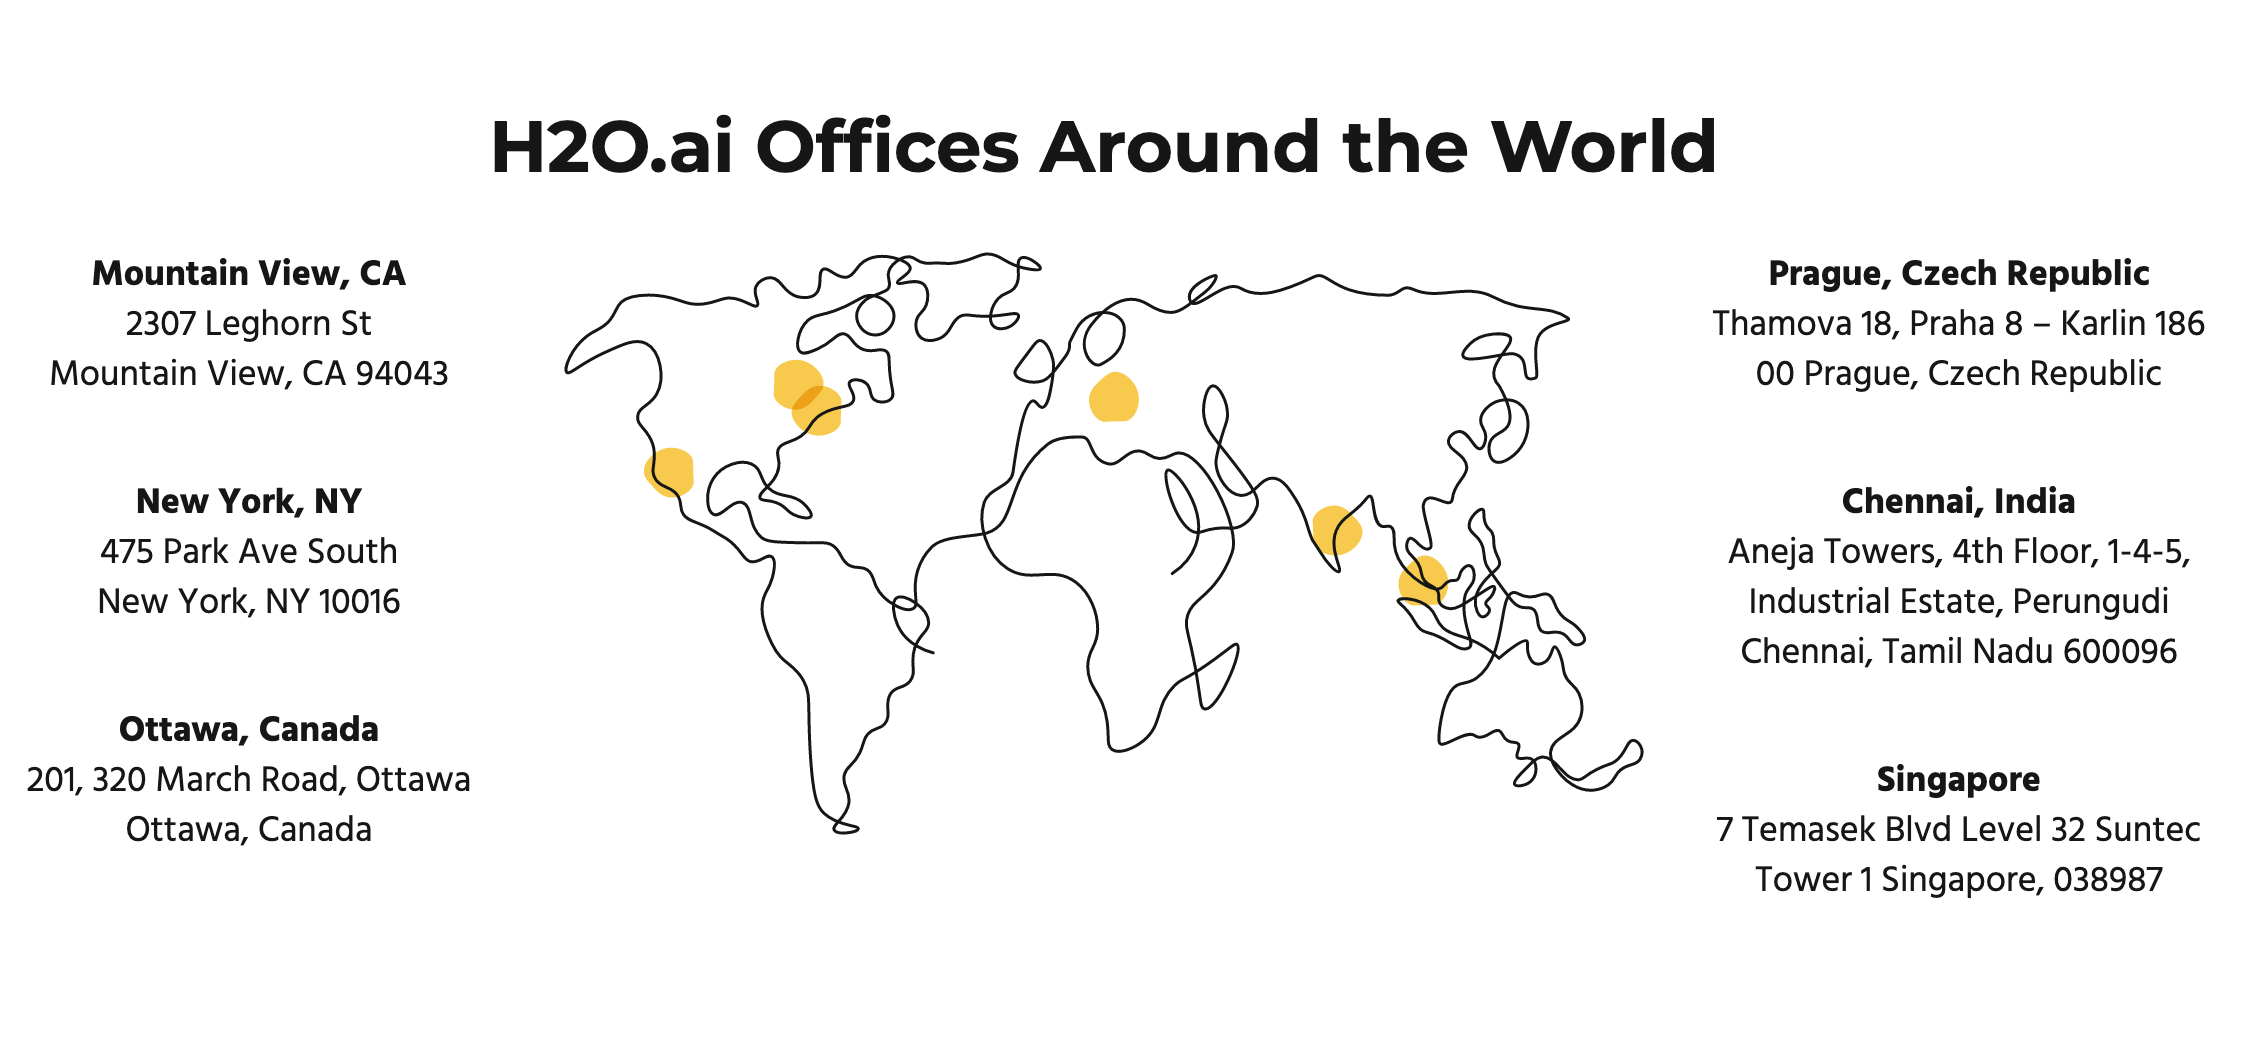
\includegraphics[width=1\textwidth]{h2oaimap.png}
\caption{H2O.ai offices around the world}
\end{figure}

% contact details hotline, emails, website, social media
H2O.ai can be contacted though the following details: \\
% centering the icons
\begin{center}

\href{https://gitter.im/h2oai/h2o-3}{ \Large \faIcon{gitter}} \ \href{https://www.linkedin.com/company/h2oai/}{ \Large \faIcon{linkedin}} \ \href{https://twitter.com/h2oai}{ \Large \faIcon{twitter}} \ \href{https://www.facebook.com/h2oai/}{ \Large \faIcon{facebook}} \ \href{https://www.youtube.com/channel/UC0ZQX4J8AmOwuGZT0IKOJyg}{ \Large \faIcon{youtube}} \ \href{https://www.instagram.com/h2oai/}{ \Large \faIcon{instagram}} \ \href{https://www.h2o.ai/}{ \Large \faIcon{globe}} \ \href{https://www.h2o.ai/contact-us/}{ \Large \faIcon{envelope}} \ \href{https://www.h2o.ai/}{ \Large \faIcon{phone}} \ \href{https://www.h2o.ai/}{ \Large \faIcon{fax}} \\

\end{center}
% add company logo
\begin{figure}[htbp]
\centering

\includegraphics[width=0.3\textwidth]{h2oai.png}
\caption{H2O.ai Logo}
\end{figure}

\section{Vision and Mission}
H2O.ai is a company that is dedicated to transforming the world through the power of \ac{AI}. The company was founded on the belief that AI should be accessible to everyone and that the power of machine learning should be accessible to people with a variety of skill sets and experiences. H2O.ai's mission is to democratize AI for everyone, everywhere. 

The company's core values are community powered, freedom to innovate, customer empathy and doing good. H2O.ai believes in being a community powered organization, where open source contributors, business leaders, nonprofits and academics can come together and collaborate to create powerful AI solutions. The company also believes in giving customers the freedom to innovate, and it works closely with the community and its customers to provide additional functionality that they need to achieve their goals. 

H2O.ai also values customer empathy, and it works tirelessly to help its customers succeed. The company understands the importance of using its knowledge and experience for good, so responsible development and model transparency are corporate-level initiatives for it. H2O.ai also seeks out opportunities in its communities where it can make a positive impact with AI.

H2O.ai's aim is to make AI accessible and easy to use for everyone. The company's mission is to democratize AI, and it is doing so by providing barrier free access to the power of machine learning. H2O.ai's core values are a testament to the company's commitment to helping its customers achieve their goals and to making a positive impact in its communities. With its focus on customer empathy and its dedication to doing good, H2O.ai is helping to make the world a better place through the power of AI.

% add journey image
\begin{figure}[htbp]
\centering
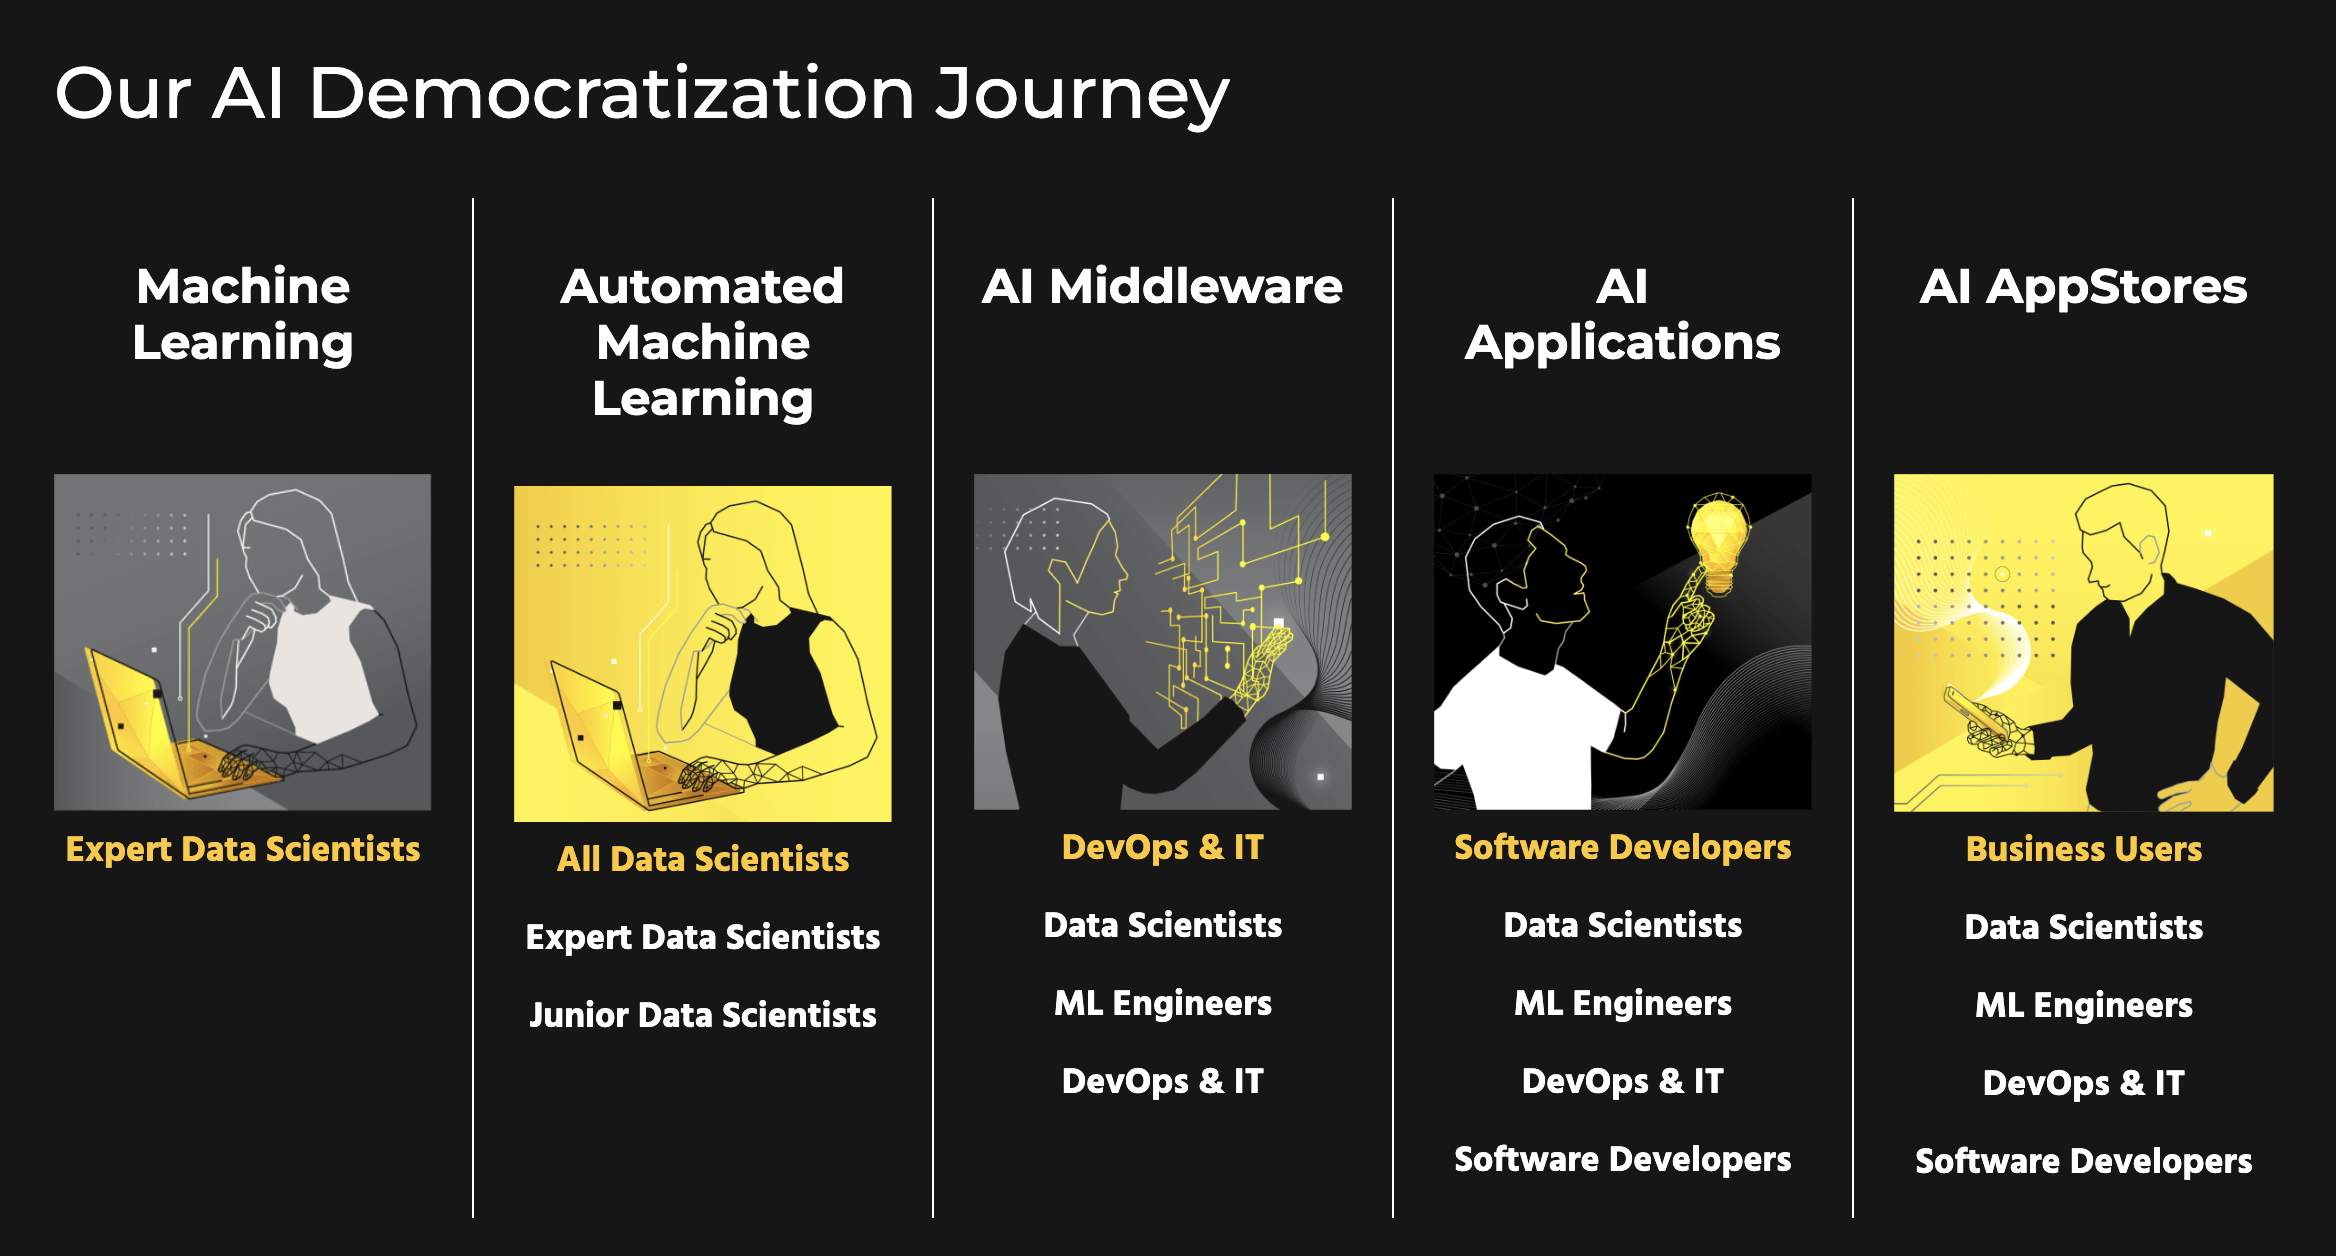
\includegraphics[width=0.8\textwidth]{journey.png}
\caption{H2O.ai Journey}
\end{figure}

\section{Organizational Structure}

In H2O.AI, There are multiple departments that work together to achieve the company's goals. The company's departments include the following: \\
\begin{itemize}
\item Product Engineering
\item Accounting and Finance
\item Business Development Representative
\item Data Science
\item Customer Data Science
\item DevOps Engineering
\item Enterprise Services
\item Exec, Sales Ops
\item Executive
\item Facilities
\item Human Resources
\item IT
\item Legal
\item Marketing

\end{itemize}

\clearpage

\subsection{Product Engineering}
H2O.AI is an enterprise-grade \ac{AI} platform that offers end-to-end AI solutions to enable organizations to accelerate and scale their AI results with trust and confidence. Its comprehensive suite of tools, services, and applications enable users to build, deploy and operate AI models quickly and easily.

H2O.AI's platform has been designed to enable a wide range of use cases, from natural language processing (NLP) and computer vision (CV) to predictive analytics, forecasting and optimization. With its unified product suite, users can quickly develop and deploy applications that are accurate, fast and transparent.

H2O.AI's product engineering team is focused on delivering AI-enabled products to customers. The team is responsible for the development and maintenance of the AI platform, and works in close collaboration with the engineering, product design, and data science teams to ensure the highest quality of product delivery. The team also works with clients to create custom solutions that meet their specific needs.

The product engineering team is composed of experienced engineers, data scientists, and product designers who are passionate about building products that are reliable, scalable, and secure. They are experienced in developing AI-based applications, and have expertise

% add org chart
\begin{figure}[htbp]
 \centering
 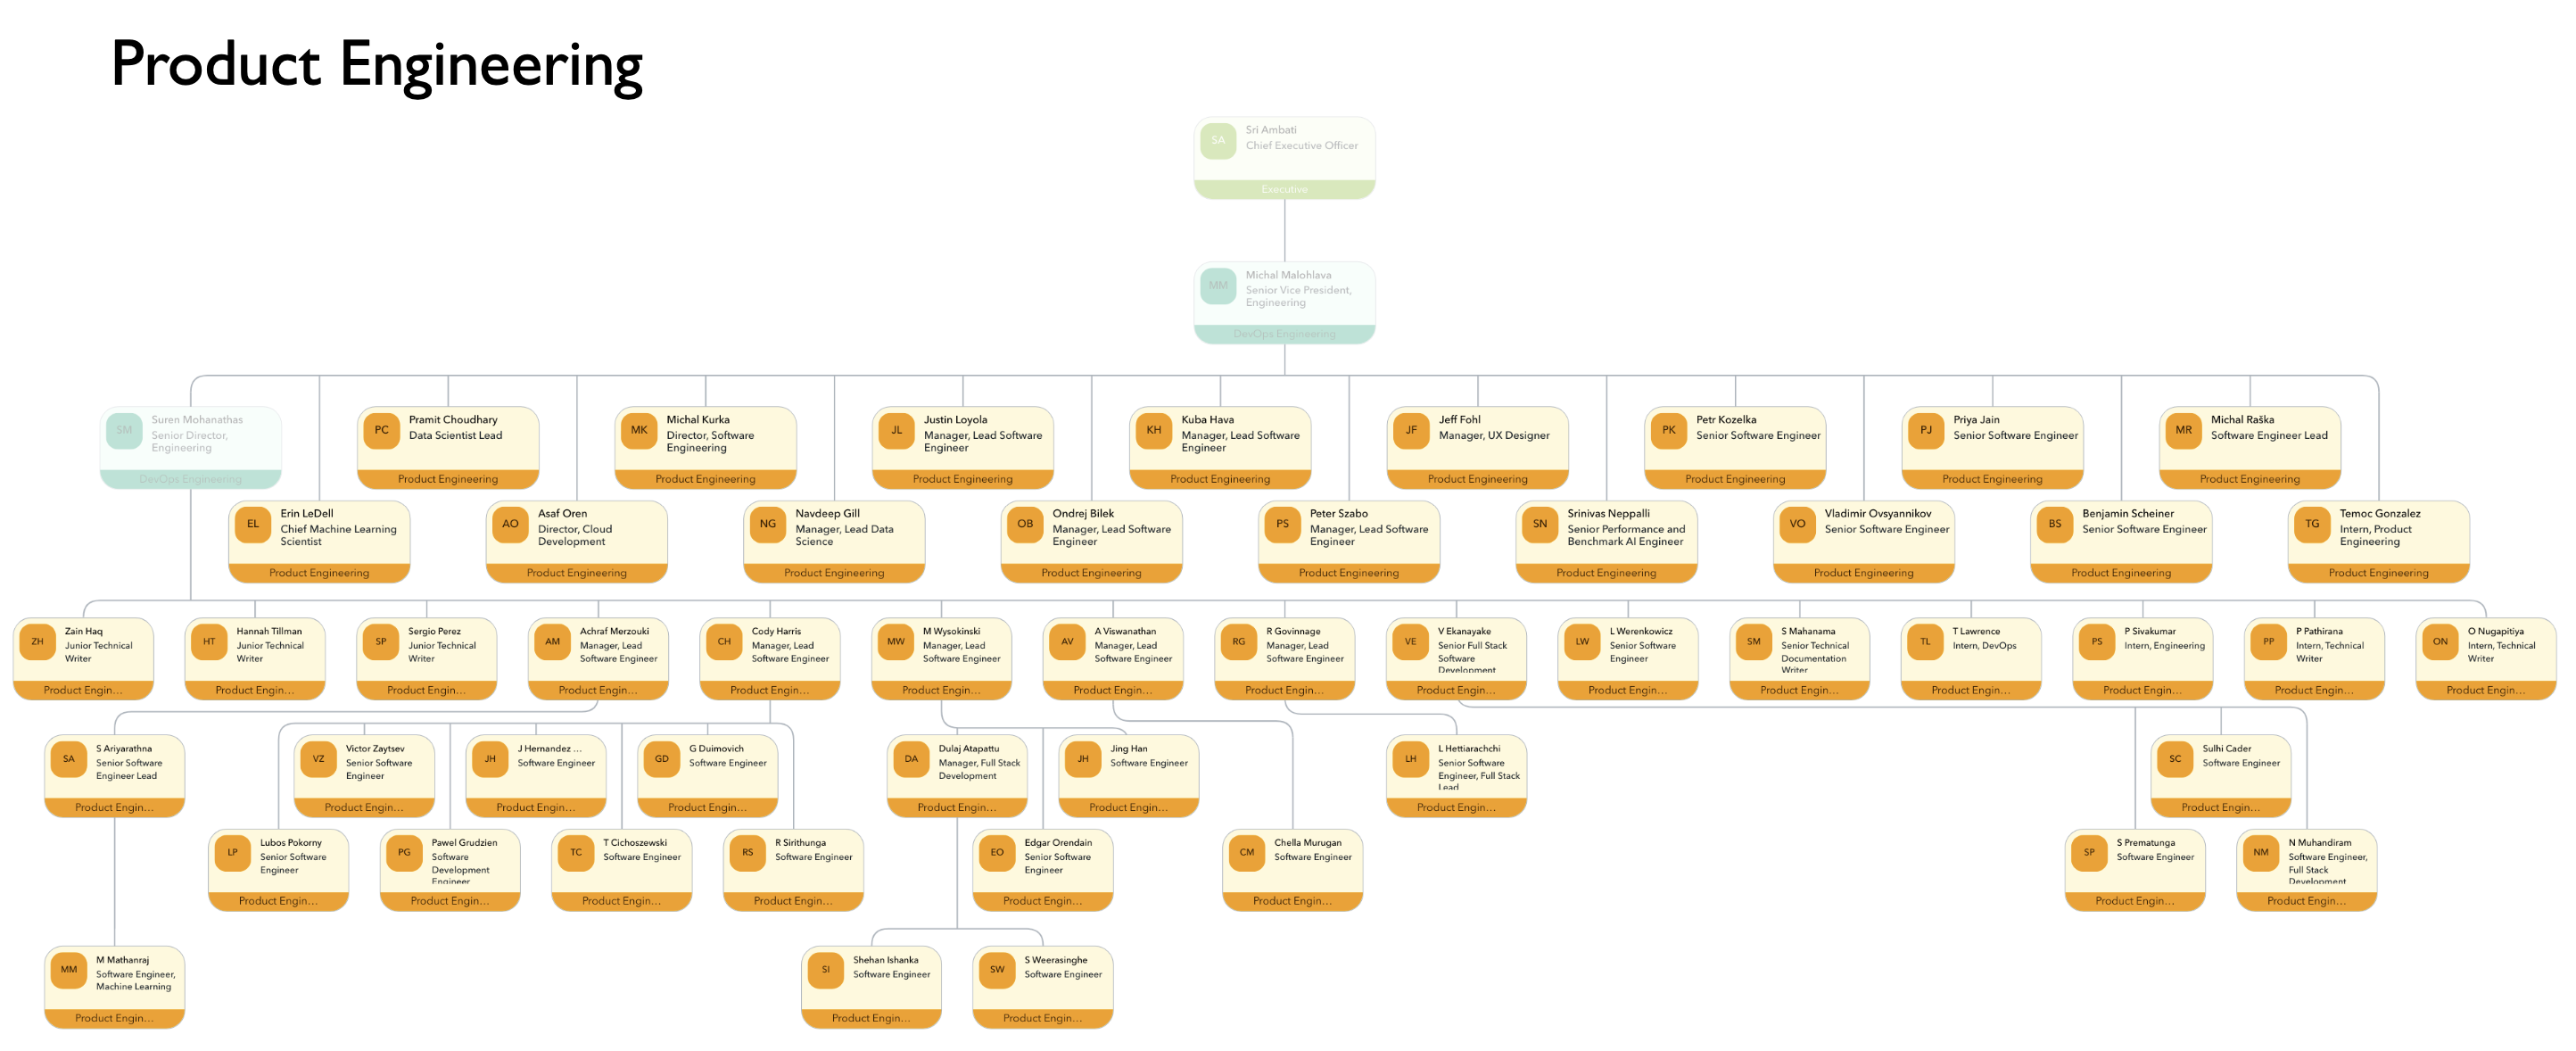
\includegraphics[width=1\textwidth]{orgchart.png}
 \caption{H2O.ai Product Engineering Organization Chart}
 \end{figure}

\clearpage
\section{Products}

\subsection{\ac{HAIC}}

% add the image haic.png
\begin{figure}[htbp]
\centering
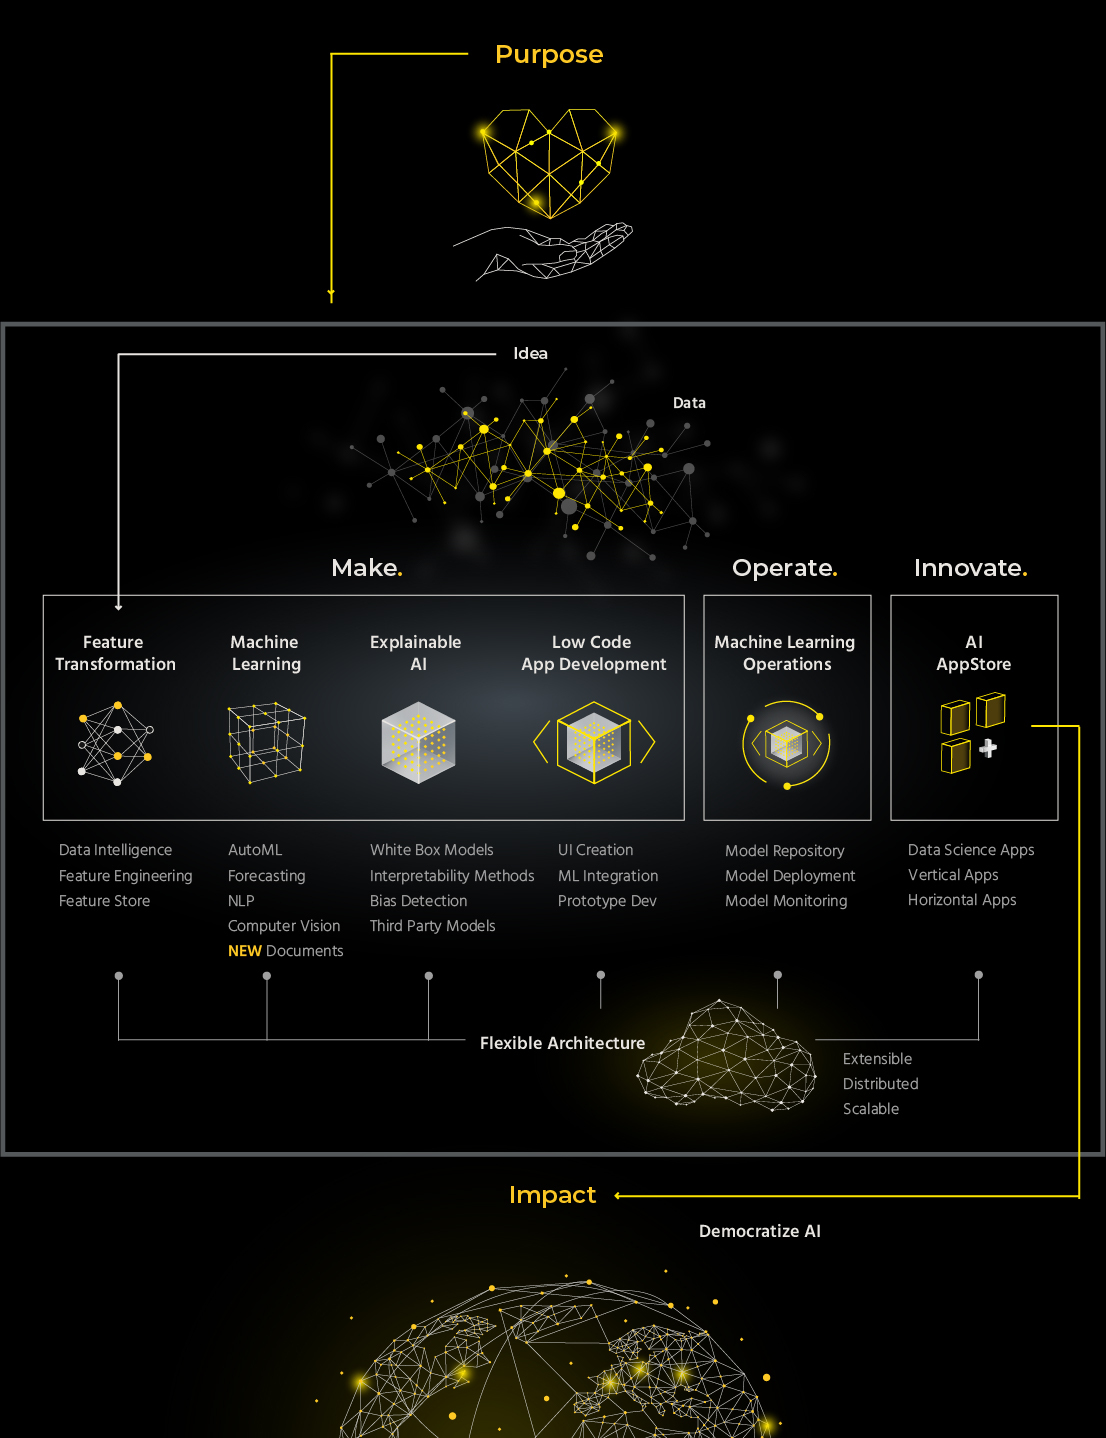
\includegraphics[width=0.9\textwidth]{haic.jpeg}
\caption{\ac{HAIC} Full Platform Capabilities\\ Their autoML capabilities have revolutionized how \ac{AI} is made and utilized. They have developed AI to carry out AI, making it simpler and quicker to use while still offering outstanding accuracy, speed, and transparency.}
\end{figure}

\ac{HAIC} is a One Platform that offers endless solutions to enable organizations to accelerate and scale their AI results with trust and confidence. Its comprehensive suite of tools, services, and applications enable users to build, deploy and operate AI models quickly and easily.

Companies around the globe are utilizing AI solutions to boost their profits, streamline processes, reduce hazards and customize consumer encounters. Additionally, numerous firms are using \ac{AI} technologies to achieve scientific advances and find new possibilities for market disruption. With the assistance of top-notch \ac{AutoML} , the \ac{HAIC} is playing an important role in helping firms to go from initial concept to actual outcomes.



These are Key Features of \ac{HAIC} 

\subsubsection{Feature Transformation}
\begin{wrapfigure}{l}{0.3\textwidth}
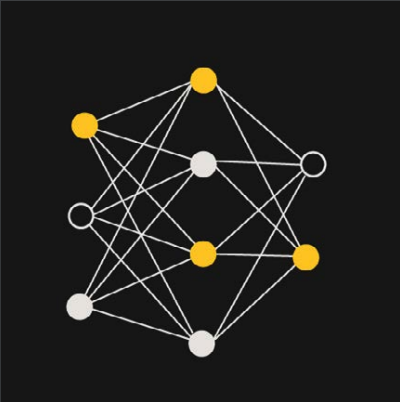
\includegraphics[width=1\linewidth]{ft.png} 
\end{wrapfigure}
Feature transformation is the process of transforming raw data into features that are more useful for machine learning algorithms. Feature transformation is a crucial step in the machine learning process, as it allows the algorithm to learn from the data more effectively. Feature transformation is also known as feature engineering, and it is a process that is used to create new features from existing ones. Feature transformation is a crucial step in the machine learning process, as it allows the algorithm to learn from the data more effectively. Feature transformation is also known as feature engineering, and it is a process that is used to create new features from existing ones.

Using Data Intelligence, They provide Data Visualization, Automatic Data Insights, Preprocessing Transformers, Dataset Splitting, Missing Value Handling, and Outlier detection.

Also in the feature engineering, They provide Automated feature engineering, Feature encoding, Feature transformation recipes, Per-Feature Controls and Automated validation and Cross validation.

In the feature store, They offer Data pipeline and Integrations, Categorization and search, Governance and access management

\subsubsection{Machine Learning}

Machine learning is the foundational element of \ac{AI} and uses algorithms to detect and extract patterns in data to predict certain outcomes based on that analysis.

\begin{wrapfigure}{r}{0.3\textwidth}
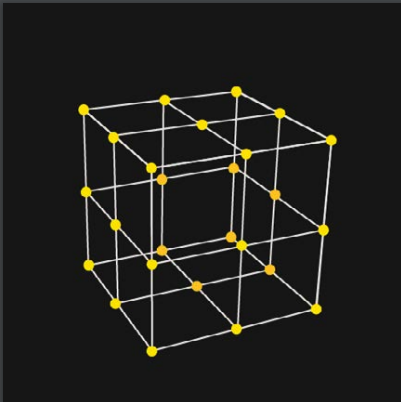
\includegraphics[width=1\linewidth]{ml.png} 
\end{wrapfigure}

\textbf{\ac{AutoML}} is the process of automating the time-consuming, iterative tasks of machine learning model development. It allows data scientists, analysts, and business users to easily build accurate models by automatically exploring thousands of possible model types and tuning parameters. AutoML is pervasive across the entire H2O AI
Cloud. Powering everything from feature transformation to model selection, monitoring
and deployment, robust autoML capabilities are the engine behind our ability to deliver
AI that does AI.

They offer Automated feature selection(dimensionality reduction), Automatic Feature Engineering, Hyperparameter Tuning, Champion/Challenger model selection, Model ensembling, Automatic label assignment, Automated model documentation, \ac{MLI} , Model Validation, Unsupervised automatic machine learning, wide dataset handling, Model Leaderboards.

\textbf{Time Series Forecasting}, Process of predicting future values based on previously observed 
values. Time series forecasting is a technique used in many fields, including finance, economics, 
and weather forecasting. Time series forecasting is a technique used in many fields, including 
finance, economics, and weather forecasting. HAIC provide Diagnostic, Leaderboard for forecasting, 
Time series \ac{MLI}.

\textbf{Natural Language Processing}, Extract insights from unstructured text data to
discover trends, create more accurate and relevant information retrieval and create
personalized recommendations. HAIC provide Text processing, Text classification, Topic clustering, 
\ac{NER}, Sentiment analysis, NLP \ac{MLI}

\textbf{Computer Vision}, Use image data for modeling with the ability to combine additional data
types with your image data to include text, tabular and audio data. HAIC provide Image processing with 
that They also provide Video processing, Audio processing, Explanation for computer vision models.

\clearpage
\subsubsection{Explainable AI}

\begin{wrapfigure}{r}{0.3\textwidth}

\includegraphics[width=1\linewidth]{exai.png}
\end{wrapfigure}

Explainable AI express the inner workings of a machine learning model in a way that is easy 
to understand. It is a technique that allows users to understand the reasoning behind the 
predictions made by a machine learning model.

\textbf{Whitebox models} are AI models which are transparent and explainable, as they are composed of 
simple functions which can be understood and studied. Such models allow for the visualization 
and explanation of the inner workings of the AI system, allowing for improved trust and understanding. Such as 
\ac{GLM}, \ac{GAM}, \ac{GA2M}, \ac{XNN}, Rulefit, Skopes Rules, Decision Trees and Linear 
model combination.

\textbf{interpretability Methods} are techniques that can be used to explain the inner workings of a
machine learning model. They are used to explain the predictions made by a machine learning model. Such as 
\ac{PDP}, \ac{ICE}, \ac{SHAP},
Feature importance, Shapley reason codes, Surrogate Decision Tree, \ac{LOCO}, k-LIME 
reason codes.

\textbf{Bias Detection} is the process of identifying and removing bias from machine learning models using 
Disparate Analysis, Sensitivity Analysis, Fairness Analysis, and Fairness Metrics.

\textbf{Third Party Models} are accepted by \ac{HAIC}. They provide a wide range of third-party models. Such as
Explanations for time series models, Explanations for computer vision models, Explanations for NLP models.
Also we can use our own models(Bring Your Own Recipe) in \ac{HAIC}.

\clearpage
\subsubsection{Low Code Application Development Framework}

\begin{wrapfigure}{l}{0.3\textwidth}

\includegraphics[width=1\linewidth]{lowCode.png}
\end{wrapfigure}

H2O.AI provide solution for rapidly building AI prototypes and applications with a low code framework using python/R that makes 
it easy y to deliver innovative solutions by seamlessly integrating backend machine learning capabilities and front end user
experiences. Also it supports machine learning integration and provides Low Code User Interface Creation Easily develop consumer
facing, interactive applications
with a Python/R framework that
supports integrated UI and AI
development.
\\

\subsubsection{Machine learning Operations(MLOps)}
\begin{wrapfigure}{r}{0.3\textwidth}

\includegraphics[width=1\linewidth]{mlops.png}
\end{wrapfigure}

MLOps is the process of managing the end-to-end lifecycle of machine learning models in production. It Automatically monitor models in real-time
and set custom thresholds to receive alerts on prediction accuracy and data drift and guarantee deployed models are operating
as intended

HAIC provide Model repository that can perform Model Management, Model versioning and 3rd Party model support.

We can also use Model deployment to deploy models in production such as Target deployment, Deployment modes and scoring.

With that, HAIC provide Model monitoring that can perform Model monitoring, Model drift detection, Model performance monitoring,
Alerts and notifications, Model governance and Model audit.

\subsubsection{Flexible Architecture}

\begin{wrapfigure}{r}{0.3\textwidth}

\includegraphics[width=1\linewidth]{flexArc.png}
\end{wrapfigure}

HAIC is environment agnostic
so any company, regardless of their
existing infrastructure, can incorporate
H2O.ai technologies into their machine
learning pipelines.

The \ac{HAIC} Flexible Architecture is an extensible and distributed platform agnostic 
platform that allows for custom recipe-based architecture, giving users the flexibility to 
train and deploy models with multiple programming languages. It is a highly scalable system 
that features NVIDIA RAPIDS integration and Ampere-based GPUs to further enhance performance. 
Additionally, \ac{HAIC} has a Platform Performance API that allows for fine-tuning of the 
AI models for maximum performance.

\ac{HAIC} has a distributed architecture that allows for multi-node training and multi-CPU/GPU 
training. It also supports Kubernetes-based deployment, offering users the capability to easily 
deploy and manage their AI models in the cloud. With this platform, users have the flexibility to 
choose the language they prefer to develop their models and train them in the cloud. The platform 
also provides support for a wide range of models, allowing users to create highly customized AI 
models tailored to their specific needs.

The \ac{HAIC} platform is designed for maximum scalability and performance. It features powerful 
hardware such as NVIDIA RAPIDS integration and Ampere-based GPUs for enhanced performance. 
Furthermore, the platform allows users to create multiple models and train them in parallel on


\subsection{H2O-3}
\begin{figure}[H]
\centering
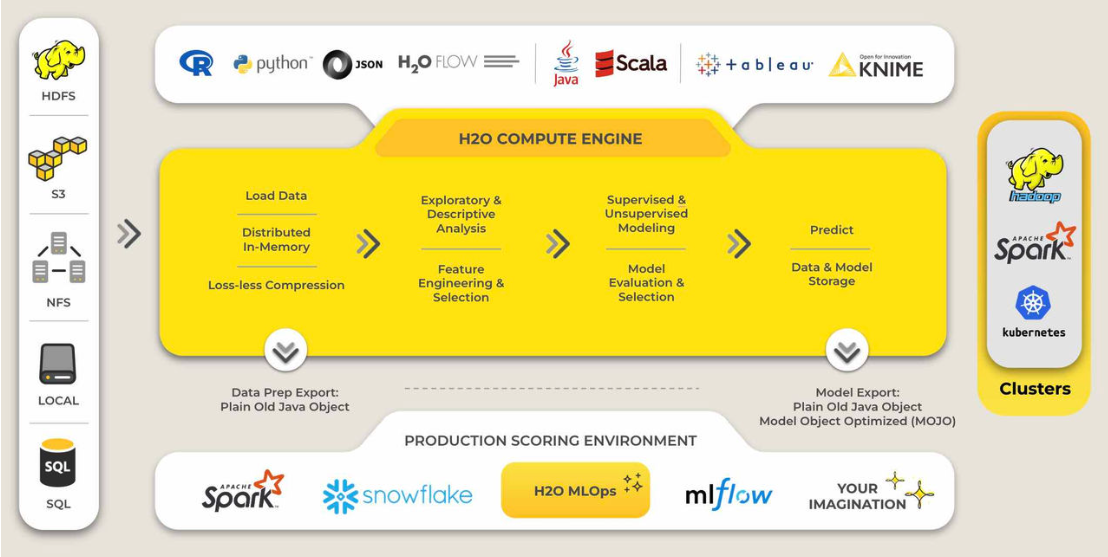
\includegraphics[width=1\textwidth]{h2o3.png}
\caption{H2O-3 Architecture}
\end{figure}


H2O-3 is a fully open source, distributed in-memory machine learning platform with linear scalability. 
H2O supports the most widely used statistical and machine learning algorithms including 
gradient boosted machines, \ac{GLM}, deep learning and more. 
H2O also has an industry leading AutoML functionality that automatically runs through all the 
algorithms and their hyperparameters to produce a leaderboard of the best models. The H2O platform 
is used by over 18,000 organizations globally and is extremely popular in both the R and Python communities.

H2O-3 can be used on existing big data infrastructure, such as Hadoop, Spark, or Kubernetes clusters, or even on bare metal. It can read data from a variety of sources, such as HDFS, Spark, S3, Azure Data Lake, and others, and store it in its distributed in-memory key-value store.


% \ac{DAI} 
\subsection{ \ac{DAI}}


\begin{figure}[H]
\centering
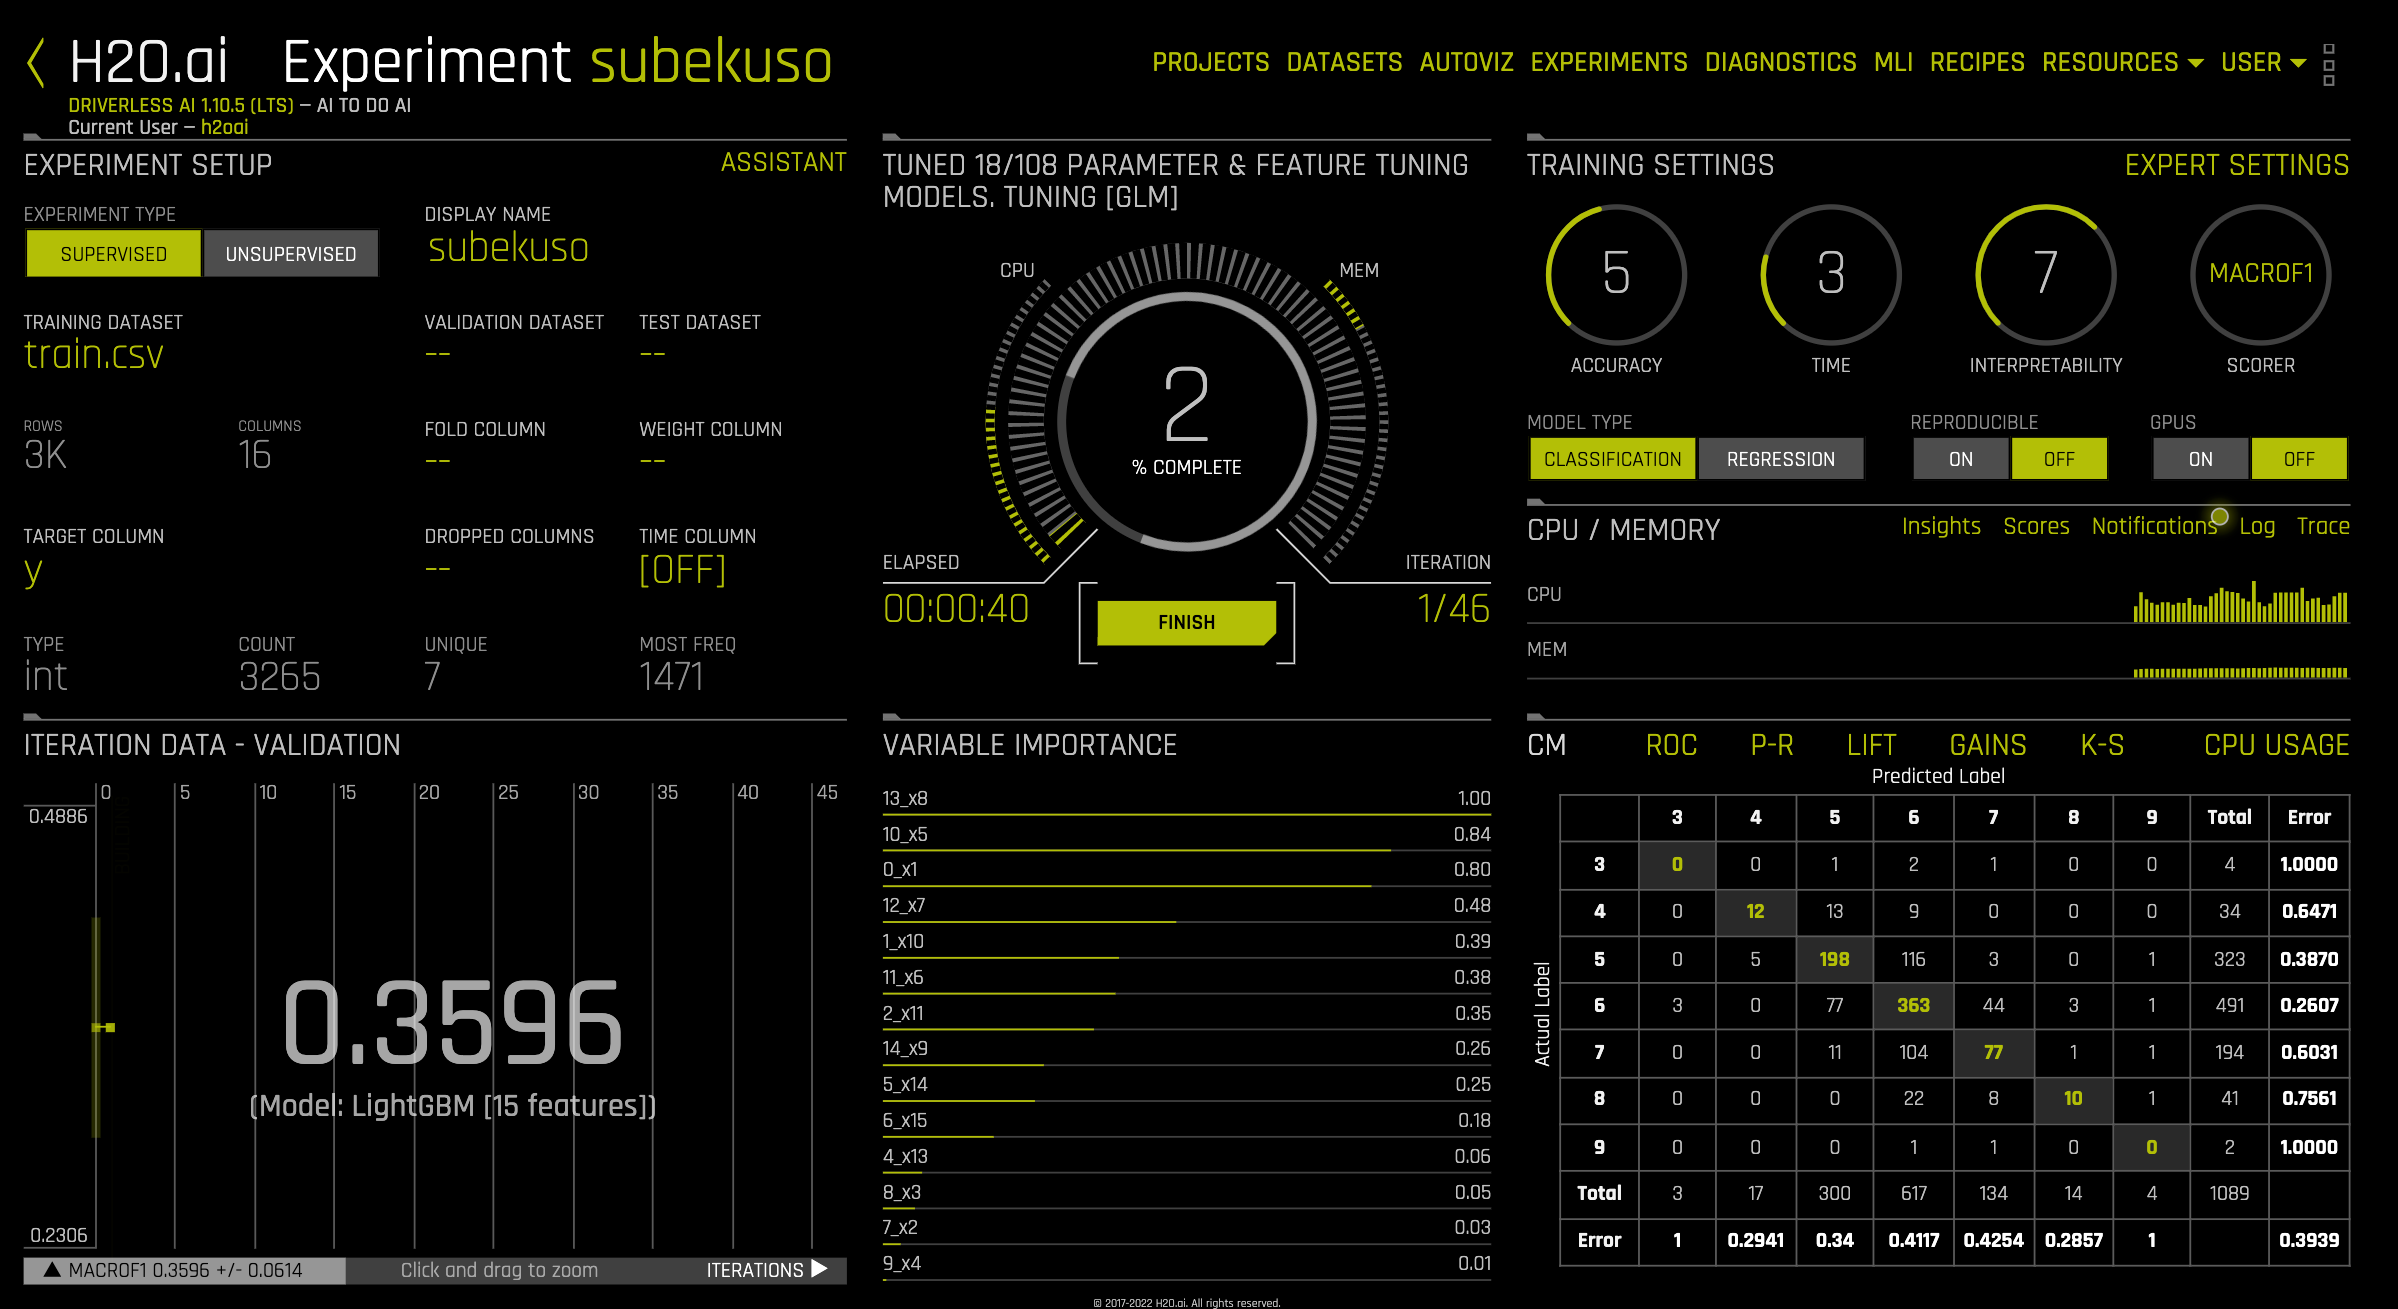
\includegraphics[width=1\textwidth]{dai.png}
\caption{ \ac{DAI} Experiment Page}
\end{figure}


 \ac{DAI} is an \ac{AutoML} platform that enables users to build, 
deploy and operate AI models quickly and easily. It is designed to enable a wide range of use cases, 
from natural language processing (NLP) and computer vision (CV) to predictive analytics, forecasting 
and optimization. With its unified product suite, users can quickly develop and deploy applications 
that are accurate, fast and transparent.

\ac{AutoML} systematically addresses multiple steps of the data science 
lifecycle with automation designed to reduce complexity across tasks and empower data scientists
to implement AI projects with higher accuracy more efficiently. AutoML also improves accessibility 
to machine learning capabilities for those without expertise in data science by providing 
user-friendly interfaces that anyone with beginner technical knowledge can use, enabling 
business users and IT professionals to easily implement machine learning into their daily workflows.

\ac{DAI} delivers industry leading autoML capabilities specifically designed to use AI to make AI, 
with automation encompassing data science best practices across key functional areas like data 
visualization, feature engineering, model development and validation, model documentation, 
\ac{MLI} and more.

\textbf{Intelligent feature transformation} H2O \ac{DAI} streamlines the feature engineering 
process by identifying relevant features in datasets, finding interactions between them, managing 
missing values, generating new features, and ranking the importance of existing and newly generated 
features. The features are transformed into values that can be easily processed by machine learning 
algorithms.

\textbf{Automated model development} Time is of the essence in the development of precise, production-ready AI models. To expedite this 
process, H2O \ac{DAI} has automated various data science tasks, such as feature engineering, 
model selection and hyperparameter tuning, and model stacking. Moreover, H2O \ac{DAI} can deploy
a low latency scoring pipeline. By leveraging both CPUs and GPUs, it is able to scan 
thousands of combinations and iterations to find the most suitable model in minutes or hours.

\textbf{Comprehensive explainability toolkit} H2O \ac{DAI} offers a comprehensive set of 
interpretability tools to help teams understand, debug, and share the results of their machine 
learning models. It features \ac{MLI} and fairness dashboards 
to help teams gain insight into their models and get a better understanding of model predictions. 
Additionally, automated model documentation and reason codes are provided for each prediction, 
allowing for greater transparency and trust in the machine learning process.

\textbf{Expert recommender system} H2O \ac{DAI} includes an AI Wizard tool that provides tailored recommendations based on your 
data and business objectives. This wizard utilizes data science best practices to ensure that 
the machine learning model created is optimized for your data and use case. It offers guidace 
on which machine learning methods are most appropriate for the given situation.

\clearpage
\subsection{H2O Wave}

H2O Wave is designed to make it easy for data scientists, machine learning engineers, 
and software developers to quickly and efficiently create interactive AI applications 
with advanced visualizations. It features a wide array of user interface components 
and charts, such as dashboard templates, dialogs, themes, widgets, and more, to expedite development.

H2O Wave run apps natively on Linux, Windows, Mac and any other operating system that supports Python.

It also run on any major cloud platform, including AWS, Azure, and Google Cloud, and can be deployed.

H2O Wave have complete flexibility and extensibility with major libraries, such as NumPy, Pandas,
and Scikit-Learn, and can be integrated with any other Python library.

\begin{figure}[H]
\centering
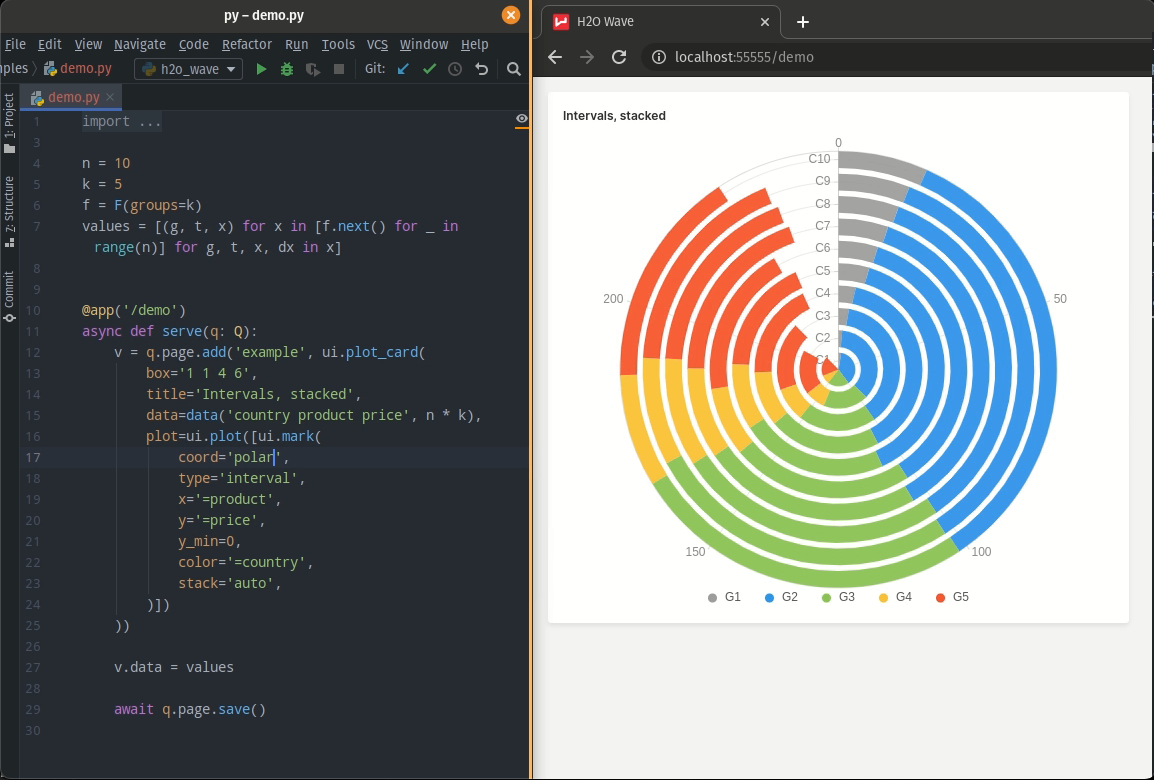
\includegraphics[width=1\textwidth]{wave.png}
\caption{Simple Wave App Development with Python}
\end{figure}

\clearpage
\subsection{H2O Document AI}

H2O Document AI is a document processing platform that enables users to extract data with Intelligence. AI can be used to automate the process of extracting key data from forms and documents, 
allowing organizations to focus on the more important elements of their operations. 
This helps to streamline processes, reduce time spent on tedious tasks, and improve 
the quality of services delivered.

\textbf{Document Processing} is the process of extracting data from documents and forms by 
scanning and creating a digital understanding of the document to allow humans to interact 
with the information it contains in a variety of ways. 


Document AI uses a combination of different machine learning techniques to help people gain 
insights from documents. These techniques include optical character recognition, 
natural language processing, handwritten text recognition, text extraction and more. By utilizing these tools, users can better understand the contents of documents, identify patterns and validate data.

\begin{figure}[H]
\centering
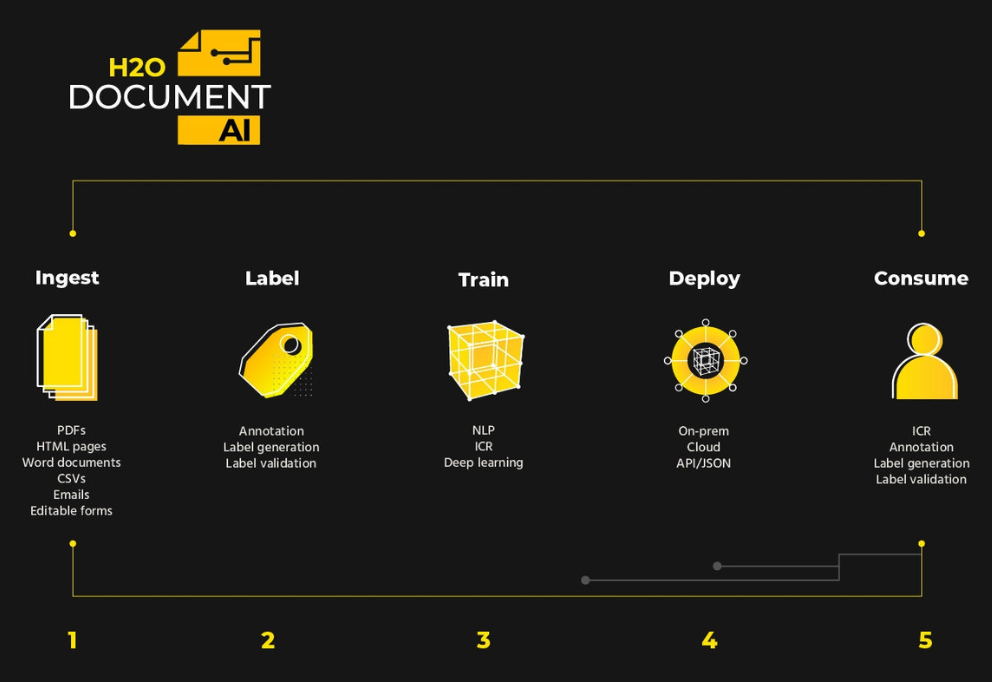
\includegraphics[width=1\textwidth]{docai.png}
\caption{Document AI How It Works}
\end{figure}


\subsection{H2O Feature Store}

H2O Feature Store is a data management platform that enables users to store, manage, 
and share features across the organization. It is designed to help data scientists 
and machine learning engineers to build and deploy machine learning models faster 
and more efficiently. It infuses data with Intelligence.

Feature engineering is the process of taking a set of independent variables, known 
as features, from a given dataset and converting them into a format that can be used
 by machine learning models to perform large-scale analysis or make predictions. 
 This process requires expertise and experience on the part of the data scientist, 
 as it can be time-consuming and requires a great deal of creativity and knowledge.
 The result of this process is a feature set that serves as the training data 
 for the machine learning model.

Feature stores address the complexity of data quality requirements by 
providing a central repository that connects information 
across disparate systems to bring all of an organization's 
data assets together in one place.


Organizations can benefit from the use of feature engineering platform that allows 
them to reuse their data and feature engineering efforts for multiple purposes. 
This platform makes it easier to store, access, manage, and share features 
for machine learning projects, leading to increased efficiency, better governance, 
and more reliable outcomes for AI initiatives.

The H2O Feature Store is designed to provide organizations with a secure and reliable 
way to store, manage, and share their data, enabling them to promote AI collaboration, 
improve operational efficiency, and ensure accuracy and reliability. The platform provides 
data security and governance with an integrated suite of tools that enable organizations 
to control who has access to what data, audit data access and changes, and maintain data 
privacy and integrity. It also helps organizations to automate data transformation and 
feature engineering processes, streamline feature pipelines for AI model training, and 
manage data versions with automated versioning. In addition, the platform provides a 
unified interface for easily discovering and understanding data, integrating with 
external data sources, and sharing data across teams and organizations. 
Finally, the platform can automate data quality assurance and monitoring 
to ensure data accuracy and reliability.

\begin{figure}[H]
\centering
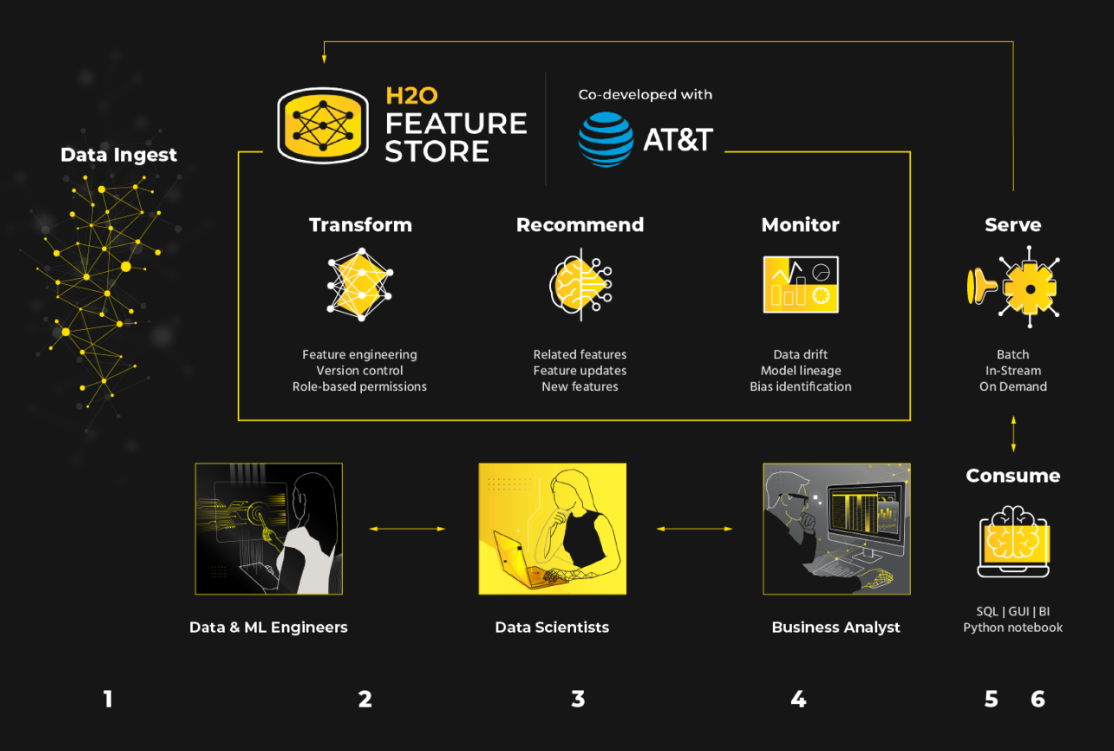
\includegraphics[width=0.7\textwidth]{fs.png}
\caption{H2O Feature Store How It Works}
\end{figure}



\section{Technology Stack}

H2O.AI uses a variety of technologies to build its products. The following is a list of the main technologies used in the development of H2O.AI products

\begin{figure}[H]
\centering
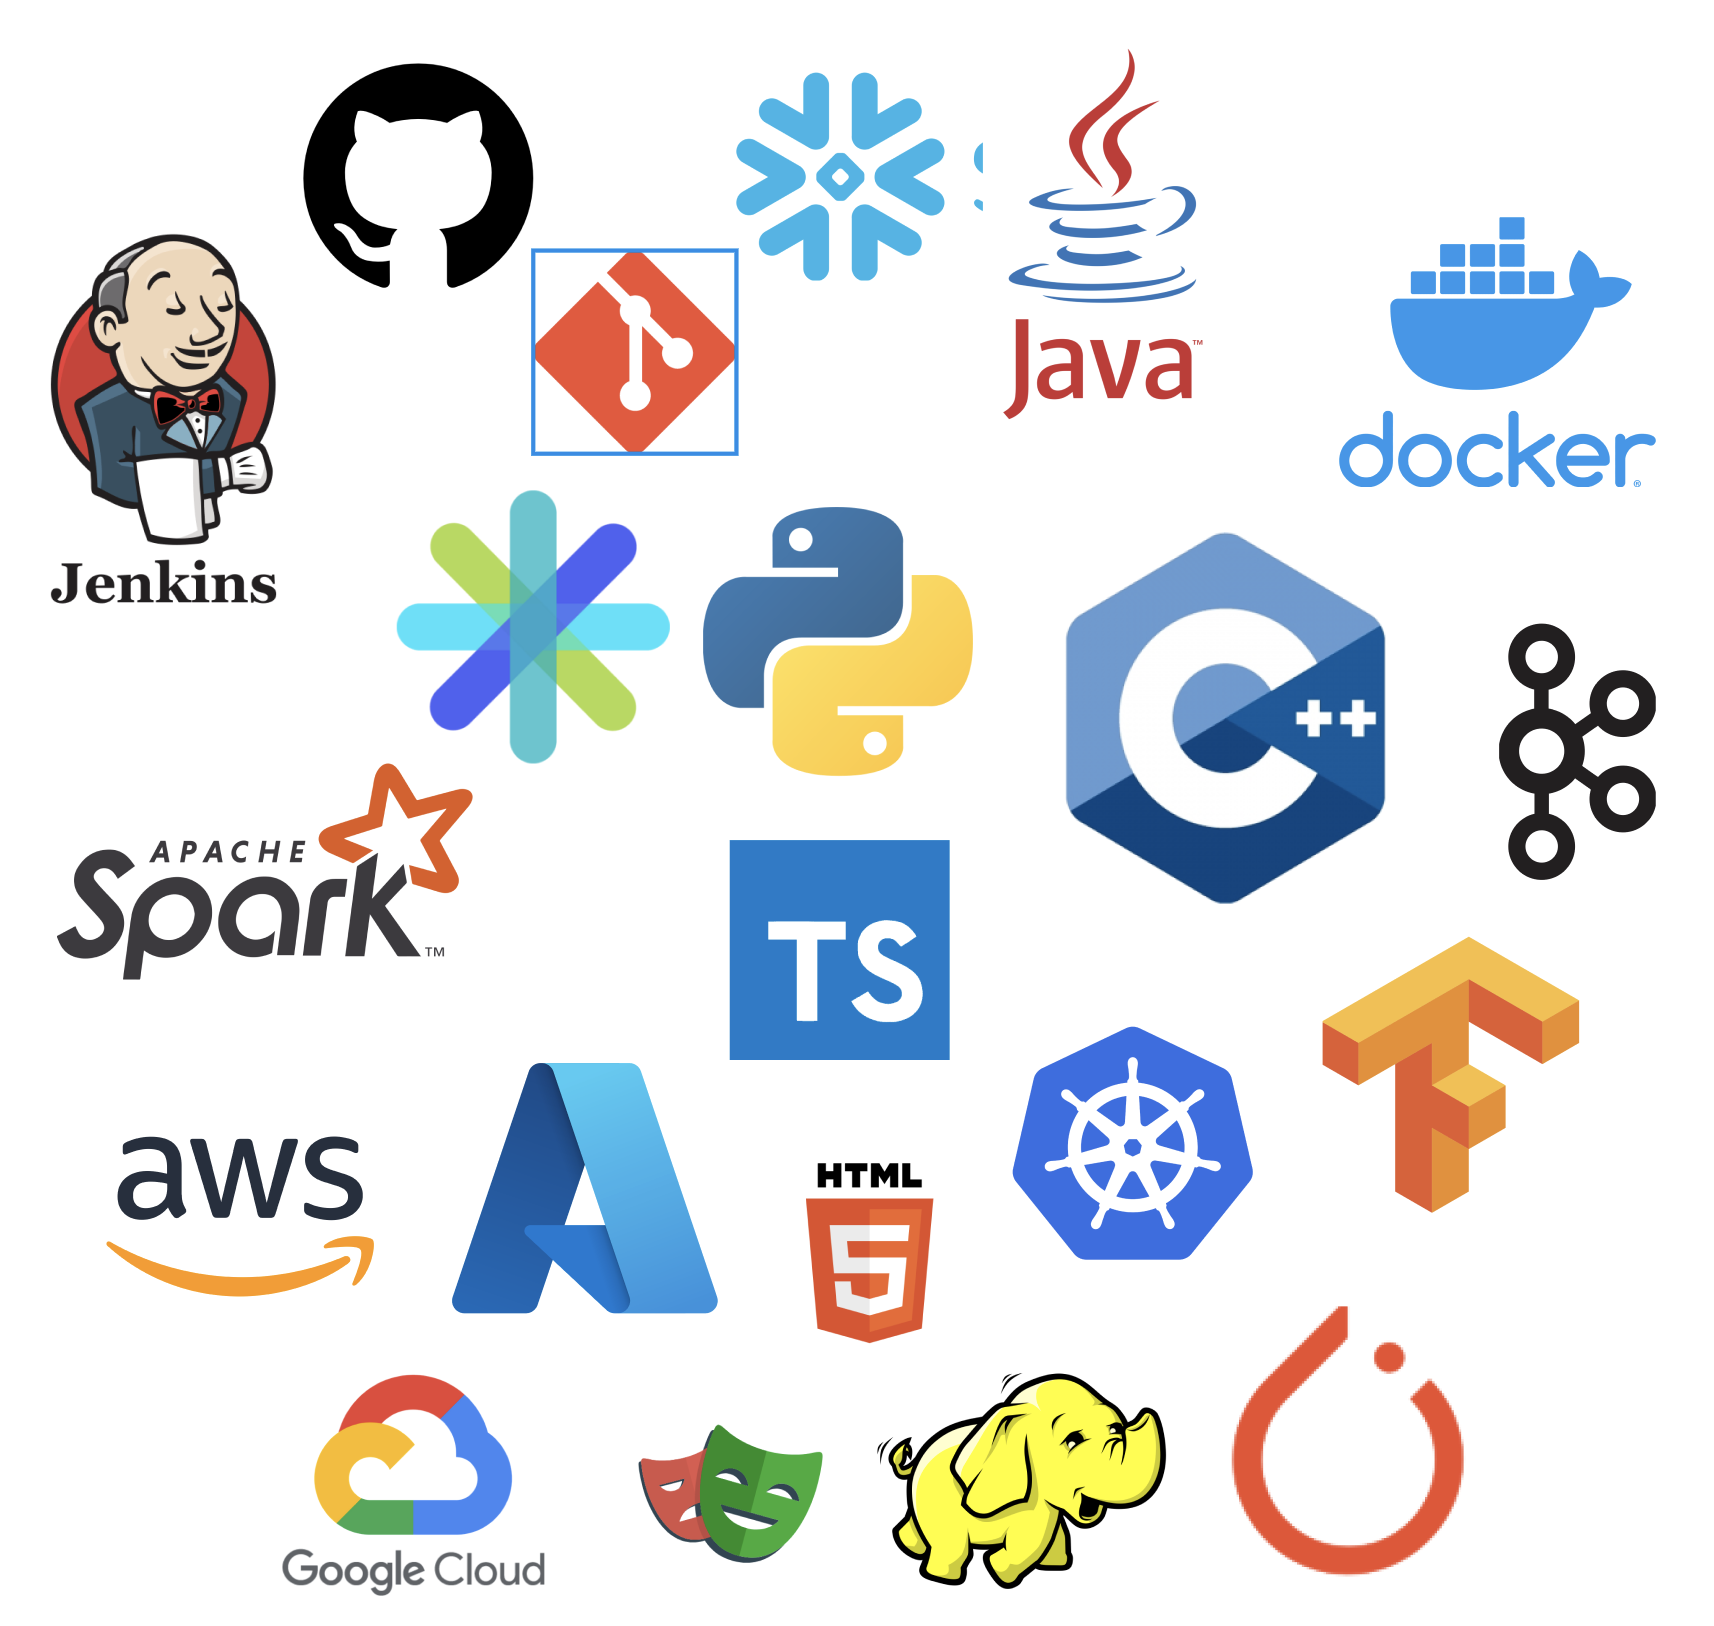
\includegraphics[width=0.7\textwidth]{techstack.png}
\caption{H2O.AI Technology Stack}
\end{figure}

\clearpage

\section{SWOT analysis}


\subsection{Strengths}
Srini Ambasti, the founder and CEO of H2O.ai, is an effective leader who has steered the company from its humble beginning to a world-class leader in \ac{AI} and machine learning. His years of experience and expertise have enabled the company to quickly become a leader in AI and ML, resulting in a company culture of innovation and dedication to excellence.

The dedicated employees at H2O.ai are a core strength of the company. They are passionate, motivated, and committed to their work, and they strive to push the boundaries of AI and ML. Through their hard work and dedication, they continue to build on the company's success.

H2O.ai is also committed to providing an environment that encourages creativity and innovation. The company's culture of collaboration and open dialogue encourages employees to think differently and generate creative solutions. This company culture has enabled H2O.ai to stay ahead of the curve in the ever-evolving landscape of AI and ML.

The company also provides a wide range of services and products that have enabled it to become a leader in the AI and ML space. H2O.ai offers a wide range of products and services, from software to hardware, from cloud services to consulting, that have enabled the company to quickly become an AI and ML leader.

The success of H2O.ai is the result of Srini Ambasti's effective leadership and the dedication of its employees. The company's culture of innovation and collaboration has enabled it to stay ahead of the curve and continue to grow. Thus, the strengths of H2O.ai are the effective leadership, dedicated employees, and company culture of innovation.

\subsection{Weakness}

One of the major weaknesses of H2O.ai is its lack of available human resources. H2O.ai is a relatively new and rapidly growing technology, and as such, there is a limited pool of experienced professionals who are familiar with the product. This can be a major obstacle when it comes to introducing the product to new clients who may be unfamiliar with its capabilities. Additionally, the lack of experienced professionals can cause problems when it comes to the implementation, deployment, and maintenance of the product. This can lead to delays in project completion and can ultimately lead to increased costs.

Another weakness of H2O.ai is the complexity of the product. H2O.ai is a powerful tool, but with great power comes great complexity. For those who are not familiar with the product, understanding how to use it effectively can be a challenge. This can lead to a steep learning curve for both new and experienced users, which can become a major obstacle for those trying to implement the product into their workflow.

Finally, H2O.ai can be expensive when compared to other similar products on the market. This is due to the fact that it is a relatively new technology and the resources required to develop, maintain, and distribute the product are high. Although the cost of the product may be worth it, it can still be a barrier for those with a limited budget.

Overall, H2O.ai is a powerful tool, but its lack of available human resources, complexity, and cost can be major weaknesses for prospective users. Those planning to use the product should be aware of these issues and plan accordingly.

\subsection{Opportunities for Improvement}

H2O.ai is a powerful machine learning platform that can be used to apply ML to a variety of areas, including the farming sector. One potential area of improvement for H2O.ai would be to create more specialized tools that are tailored to the needs of the farming sector. For example, H2O.ai could develop software that is specifically designed to help farmers with their crop planning, decision-making, and management. This could include predictive models for predicting crop yields, forecasting weather, and predicting market prices. 

Another potential area of improvement could be to expand the range of datasets available for use with H2O.ai. Currently, the datasets available are limited to certain fields such as finance, marketing, and retail. By adding datasets specifically related to farming, H2O.ai could be used to create more accurate models and insights. Additionally, H2O.ai could also focus on developing tools that take into account the unique characteristics of farming such as soil and climate conditions.

\subsection{Threats for Survival}

H2O.ai is a powerful tool for machine learning and \ac{AI}. It offers a great platform for data scientists to quickly build and deploy models with minimal effort. However, there are some threats that can hinder the improvement of H2O.ai. 

The first threat is the lack of data scientists. H2O.ai offers powerful tools, but it requires a certain level of expertise to use them. Without enough data scientists, the platform may not be able to take full advantage of its capabilities.

The second threat is the risk of data leakage. As the platform is used to store and process large amounts of data, there is a risk of data leakage due to malicious actors or security breaches. This could lead to the loss of sensitive information and the potential for financial losses.

The third threat is the lack of scalability. H2O.ai is great for small-scale applications, but it is not always suitable for large-scale tasks. This could limit its potential for improvement.

The fourth threat is the need for continuous updates. As new technologies are developed, the platform needs to be updated to remain competitive. This requires a lot of time and effort, and it could be difficult to keep up with the pace

\chapter{Training Experience}

This chapter describes the training experience at H2O.ai. It includes the training process, the training materials, and the training environment.


\section{Working hours}
At H2O.ai, employees are expected to work 40 hours per week, with flexibility to adjust as needed. The company encourages employees to take time off to rest and recharge, and provides generous vacation, sick, and personal time off benefits. The company also offers flexible working arrangements, such as remote work, compressed workweeks, or part-time hours, to accommodate individual needs.

H2O.ai encourages open communication and collaboration, and provides an environment where employees feel supported and respected. The company promotes a culture of innovation and offers a wide range of learning and development opportunities to help employees grow professionally.

To further promote a positive work environment, H2O.ai encourages employees to get involved in the company's activities, such as volunteering, mentoring, attending company events, and more. The company also offers various employee appreciation programs, such as team-building activities and recognition awards.

H2O.ai is committed to fostering an inclusive and diverse workplace, and is continually looking for ways to improve its working environment for employees. The company is committed to providing equal opportunities for all employees and encourages everyone to give feedback and suggest ways in which the company can improve. Through its focus on openness and inclusivity, H2O.ai strives to create a workplace that is comfortable for all.

\section{Team}

The team at H2O.ai is made up of a diverse group of individuals with a wide range of 
skills and experience. The team is led by Srini Ambasti, the founder and CEO of H2O.ai, 
who has over 20 years of experience in the field of \ac{AI} and machine learning. 
The team also includes a number of data scientists, software engineers, and product managers 
who are dedicated to the company's mission of making AI and ML accessible to everyone.

\subsection {Product Engineering Team}
H2O.ai's product engineering teams are responsible for developing, testing, and maintaining the company's software products. This includes the development of core machine learning algorithms, the implementation of user-friendly applications, and the management of the product's underlying infrastructure.

The product engineering teams use a variety of tools and technologies to ensure that the products they build are of the highest quality and meet customer needs. The teams practice \ac{CI} to ensure that the code they develop is tested and released frequently. This helps reduce the time it takes to release a product and makes sure that bugs are identified and resolved quickly. The teams also use \ac{CD} to ensure that the product is deployed quickly and safely to customers.

The teams also work closely with other departments, such as product management and customer success, to ensure that the product meets customer needs and is delivered on time. The teams are also responsible for ensuring that the software is secure and compliant with industry standards.

The product engineering teams use a variety of techniques to keep the code clean and maintainable. This includes using \ac{VCS}s, writing automated tests, and using code reviews to ensure that the code is of the highest quality. The teams also use automated deployment tools to make sure that the software is released quickly and safely.

In short, H2O.ai's product engineering teams are responsible for developing, testing, and maintaining the company's software products. They use a variety of tools and techniques to ensure that the products are of the highest quality and meet customer needs. The teams also work closely with other departments to make sure that the product is delivered on time and is secure and compliant with industry standards.

Each products have their own team. For example, the \ac{DAI} team is responsible for developing, testing, and maintaining the \ac{DAI} product. The \ac{DAI} team uses a variety of tools and techniques to ensure that the product is of the highest quality and meets customer needs. The team also works closely with other departments to make sure that the product is delivered on time and is secure and compliant with industry standards.

Since \ac{DAI} is flagship product, it has the most resources and the most people. The team is divided into several sub-teams, each with their own responsibilities. For example, the \ac{DAI} team is responsible for developing, testing, and maintaining the \ac{DAI} product. The \ac{DAI} team uses a variety of tools and techniques to ensure that the product is of the highest quality and meets customer needs. The team also works closely with other departments to make sure that the product is delivered on time and is secure and compliant with industry standards.
I am working on the \ac{DAI} team for 6 months to automate the GUI testing. My dedicated Team was 3 People including me. One is Jiri Puc who is Full Stack Engineer and Other one is Joby who is QA Engineer.

% add jiri and joby images parallel to each other
\begin{figure}[H]

\begin{subfigure}[h]{0.5\textwidth}
\centering
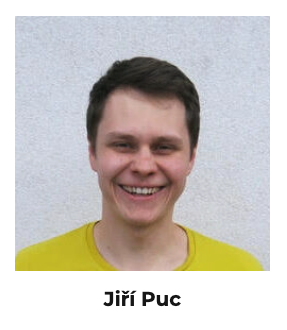
\includegraphics[width=0.9\linewidth]{jiri.png}
\end{subfigure}
\hfill
\begin{subfigure}[h]{0.5\textwidth}
\centering
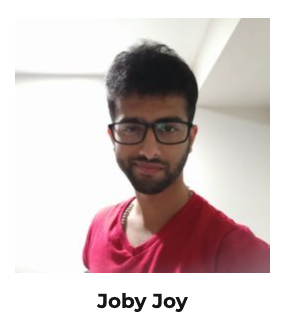
\includegraphics[width=0.9\linewidth]{joby.png}
\end{subfigure}

\caption{\ac{DAI} \ac{GUI} and Testing Team}
\end{figure}

\subsection {Data Science Team}

The Data Science Team at H2O.ai focuses on building industry-leading \ac{AI} and machine learning solutions. The team consists of experienced data scientists and engineers who are passionate about data and its potential to transform businesses. The team works on applied and fundamental research, engineering, product development, and customer engagement. The team is responsible for developing H2O's advanced machine learning and \ac{AI} platforms, as well as its applications and products. The team's mission is to make data science more accessible, easier to use, and more powerful for everyone.

Along with product engineering works, I also worked as a data scientist intern at H2O.ai, with Shivam Bansal who is a Kaggle Grand Master. Together, we work on projects that involve analyzing and interpreting complex data sets to gain insights and develop solutions. We utilize advanced machine learning and \ac{AI} techniques such as deep learning and neural networks to develop predictive models that can be used to make predictions or classify data. Our work also involves developing and implementing data visualizations to present data in a meaningful way. We collaborate closely to ensure that our solutions are optimized to meet the customer's needs.

% add shivam 
\begin{figure}[H]
\centering

\includegraphics[width=0.5\linewidth]{shivam.png}
\caption{Data Science Team}
\end{figure}

\section{Working procedure}

Since I am working multiple teams at H2O.AI, I follow a process that allows me to work effectively and efficiently, whether it's in the office or remotely. To begin with, I prioritize my workload and make sure to focus on the tasks that are most important and urgent. This ensures that I stay productive and efficient while ensuring that I don't miss any deadlines. I use various tools to keep organized, like task lists and calendars. This helps me to keep track of tasks, deadlines, and progress.

I also make sure to stay in communication with my team, whether it be via email, Slack, or in-person meetings. This allows us to collaborate effectively and catch any potential issues before they become problems. In addition, I stay aware of time differences when working with people in different time zones. If necessary, I adjust my schedule to accommodate for this, so that I can maintain effective communication with everyone.

Finally, I make sure to use best practices when working remotely. This includes using secure networks, using encryption when necessary, and using two-factor authentication when accessing sensitive data. By following these processes, I am able to work effectively, efficiently, and securely at H2o.ai.

\subsection*{Life cycle of \ac{DAI}}

\ac{CI} and \ac{CD} are important principles in the development of \ac{DAI} in H2O.ai. CI/CD\cite{noauthor_what_nodate} is an automated process of integrating and delivering changes from development to production. It helps to reduce the time and cost of development, as well as increase the quality of the product.

CI/CD starts with the developer checking out code from the repository and adding it to the local development environment. This code is then tested for bugs and other issues. Once the code is ready, it is committed to the repository and an automated process is used to build and deploy it.

\begin{figure}[H]
\centering
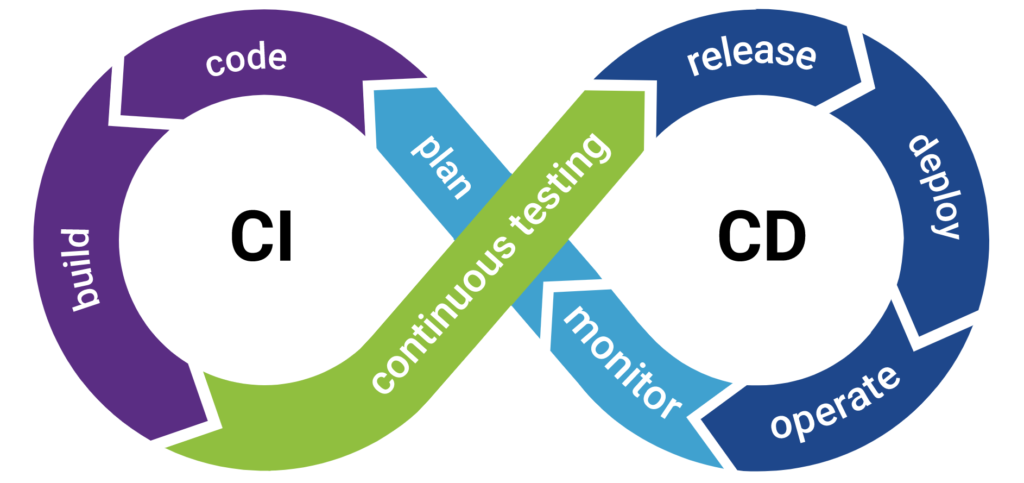
\includegraphics[width=0.5\linewidth]{cicd.png}
\caption{CI/CD}
\end{figure}

The automated process consists of several steps. First, the code is built and tested against the unit tests and integration tests to ensure that the code is working correctly. If the tests pass, the code is packaged and deployed to production. After the deployment, a series of end-to-end tests are run to ensure that the code is functioning correctly in the production environment.

Finally, after the code is tested and deployed, the changes are monitored. This includes tracking errors, performance metrics, and user feedback. If any issues are found, they are addressed and fixed as soon as possible.

CI/CD helps to ensure that the code is production-ready and that it works as expected. This helps to reduce the time and cost of development, as well as increase the quality of the product. It also helps to ensure that the code is always up-to-date and that any changes are tested and deployed quickly.

\subsection*{Data Science Life Cycle}

At H2O.ai, data scientists use the H2O.ai platform to build data-driven solutions for their clients. The H2O.ai platform is an open source platform for machine learning, deep learning, and predictive analytics.

The first step in the H2O.ai data scientist work cycle is to collect and organize data. This includes gathering, cleaning, and building data sets from a variety of sources, such as databases, CSV files, and APIs. Data scientists will then use data exploration and visualization techniques to gain an understanding of the data and identify patterns.

The next step is to create and evaluate models. Data scientists use H2O.ai's \ac{AutoML} feature to quickly generate and test multiple models in order to find the best performing one. They also utilize feature engineering techniques to further refine the models.

Once the best model is identified, the data scientists deploy the model into production. This involves setting up a secure environment, creating a server to host the model, and setting up the necessary APIs to access the model.

The final step is to monitor and maintain the model. This includes tracking model performance, updating the model when necessary, and ensuring the model is secure. Data scientists

\section{Tools used}

During my internship at H2O.ai, I used a variety of tools and technologies to complete my work such as \ac{IDE} , \ac{VCS} , \ac{CI} and \ac{CD} ... etc. 

\subsection{\ac{IDE}}

\begin{wrapfigure}{l}{0.2\textwidth}

\includegraphics[width=1\linewidth]{vscode.png} 
\end{wrapfigure}

Visual Code\cite{noauthor_visual_nodate} as \ac{IDE} is an open source tool developed by Microsoft for editing, debugging and developing programs. It supports hundreds of programming languages, including Python, JavaScript and C++. It provides features such as code completion and refactoring, code linting, and integrated debugging. Visual Code is used by developers to develop and debug \ac{DAI} models.
\\

\subsection{\ac{VCS}}


\begin{wrapfigure}{r}{0.3\textwidth}

\includegraphics[width=1\linewidth]{git.png} 
\end{wrapfigure}

Git is a \ac{VCS} used to track changes in source code. It allows developers to collaborate on projects and share code with each other. Git is used by developers to version and store \ac{DAI}.

Github is a web-based \ac{VCS} used to store and manage source code. It allows developers and data scientists to collaborate on projects and share code with each other. \ac{DAI} can be stored and versioned in GitHub repositories.

\subsection{Content Management Tools}

\begin{wrapfigure}{l}{0.2\textwidth}

\includegraphics[width=1\linewidth]{confluence.png}
\end{wrapfigure}

Confluence is a collaboration platform used to share information and collaborate on projects. Confluence helps to share documents, notes and ideas related to their \ac{DAI} projects.
It also contain every information about the project and the team members. License of products, Terms and conditions, and other important information are also available in Confluence.
\\
\subsection{User Interface Framework}

\begin{wrapfigure}{r}{0.3\textwidth}

\includegraphics[width=1\linewidth]{h2o-flow.png}
\end{wrapfigure}

We use H2O Flow created by H2O.ai to create the user interface for \ac{DAI}. H2O Flow is a web-based \ac{GUI} for the H2O machine learning platform. It enables users to build and manage machine learning models, tune hyperparameters, and visualize model performance and results. With H2O Flow, users can quickly and easily explore, analyze, and build sophisticated machine learning models and pipelines. H2O Flow also provides users with access to high-level algorithms, such as gradient boosting and deep learning, as well as low-level APIs for more advanced users. Additionally, H2O Flow offers a wide range of interactive visualizations and data exploration tools, making it easy to explore data and build models.

\subsection{Cloud Computing Platform}

\begin{wrapfigure}{l}{0.2\textwidth}

\includegraphics[width=1\linewidth]{aws.png}
\end{wrapfigure}

\ac{AWS}\cite{noauthor_cloud_nodate} is a cloud computing platform that provides a wide range of services, including virtual machines, storage and databases. \ac{DAI} models can be deployed to AWS infrastructure for production use. S3 bucket is used to store the data and models. EC2 instance is used to run the \ac{DAI} model. EC2 instance is a virtual server in the cloud. It is a web service that provides secure, resizable compute capacity in the cloud. It is designed to make web-scale cloud computing easier for developers. EC2 instance is used to run the \ac{DAI} model. 

\subsection{Automation Tools}

\subsubsection*{Jenkins}

\begin{wrapfigure}{r}{0.3\textwidth}

\includegraphics[width=1\linewidth]{jenkins.png}
\end{wrapfigure}

Jenkins\cite{noauthor_jenkins_nodate} is a \ac{CI} system used for automation and deployment of software applications. With the help of Jenkins, businesses can easily and quickly build, test, and deploy software applications. \ac{DAI} is an \ac{AutoML} platform that uses advanced AI algorithms to automate the process of building and deploying machine learning models. Jenkins is used in \ac{DAI} to automate the code building process, test it, and deploy it to the production environment. With Jenkins, developers can easily configure a job to automatically build the code and deploy it to the production environment. This process helps to reduce the time taken to manually build and deploy the code. Furthermore, Jenkins can also be used to monitor the code in the production environment and alert developers if any errors occur.

In addition to automating the code building and deployment process, Jenkins can also be used in \ac{DAI} to automate the machine learning model building process. Jenkins can be used to schedule automated jobs to build and deploy machine learning models. The automation process makes it easier for businesses to quickly build and deploy machine learning models in a short amount of time. Furthermore, Jenkins can also be used to monitor the performance of the machine learning models in the production environment, alerting developers of any changes or errors that may occur.

Overall, Jenkins is an effective tool for automating the code building, deployment, and machine learning model building processes in \ac{DAI}. With Jenkins, businesses can quickly and easily build, test, and deploy applications in a short amount of time. Furthermore, Jenkins can also be used to monitor the code and machine learning models in the production environment, alerting developers of any changes or errors that may occur.

\subsubsection*{Playwright}

\begin{wrapfigure}{l}{0.2\textwidth}

\includegraphics[width=1\linewidth]{playwright.png}
\end{wrapfigure}

Playwright\cite{noauthor_fast_nodate} is an automated testing library designed and maintained by the Microsoft Edge team. It provides a unified API for scripting and automating interactions with web applications. It is used in \ac{DAI} GUI to automate the testing of user interfaces for web applications. Playwright helps to simulate user interactions such as clicking, typing, selecting, and dragging. It also enables the automation of webpages, allowing for quick and easy testing of user interfaces. It can be used to test the user experience across different browsers and devices, helping to ensure consistent performance and usability. 

Playwright also enables the automation of the testing of \ac{DAI} GUI. It can be used to simulate the navigation of the GUI, the selection of the menus, and the triggering of the commands. This makes it easier to test the functionality of the UI and to ensure that it works as expected. It also helps to identify potential bugs or issues in the GUI before they are released. Playwright also helps to automate regression tests, which can help to identify any issues or problems that may arise due to changes in the code. It is also capable of testing the performance of the GUI, helping to ensure that it is responsive and usable. This is especially important for the automation of \ac{DAI} GUI

\subsection{Communication Tool}

\subsubsection*{Slack}

\begin{wrapfigure}{r}{0.2\textwidth}

\includegraphics[width=1\linewidth]{slack.png}
\end{wrapfigure}

Slack is a collaboration platform designed to help teams communicate and collaborate more effectively. It provides a single place for teams to share information, communicate, and stay organized. With Slack, teams can communicate in real-time, share documents and files, and have private conversations. Slack is especially effective for teams that are working remotely or have different locations. It makes it easy to keep everyone on the same page, regardless of their location. Slack allows users to create channels for specific topics or conversations, and they can be public or private. This makes it easy to organize conversations and keep them focused on the task at hand. Slack also offers many features to help teams collaborate more efficiently. It includes tools for task management, document sharing, and project management. This helps teams stay organized and on top of their tasks. Additionally, Slack has integrations with other services, such as Dropbox, Google Drive, and more, which makes it even easier to keep track of all the different tasks and conversations.

Slack also has mobile and desktop apps, which make it easier to stay connected and collaborate with team members. The mobile app enables users to check notifications, send messages, and access files from anywhere. The desktop version has a similar set of features, so users can stay productive even when away from their desks.

Overall, Slack is a great tool to help teams collaborate and stay organized. It makes it easy to stay connected and organized, regardless of location. Slack is also very user-friendly and has a variety of features to help teams stay productive.
\subsubsection*{Zoom}

\begin{wrapfigure}{l}{0.2\textwidth}

\includegraphics[width=1\linewidth]{zoom.png}
\end{wrapfigure}

Zoom is a cloud-based video conferencing platform that enables users to collaborate virtually with colleagues, partners, and customers from any location. Zoom is a great tool for remote teams to use for collaboration. It allows for easy and fast set up of video conferences, and it also provides an easy way for users to share and collaborate on documents. Zoom has several features that make it great for collaboration. For starters, it has a screen-sharing feature which allows users to share their screen with other participants in the meeting. This is great for brainstorming and sharing ideas. Additionally, Zoom allows users to record their meetings, which is a great way to review the content of a meeting afterwards.

Furthermore, Zoom allows users to chat with each other in a group chat or directly with each other. This makes it easy to discuss topics in more detail or ask questions. It also allows users to share files with each other and collaborate on documents in real-time. This feature is particularly useful for teams who are working on a project together.

Overall, Zoom is a great tool for collaboration. It has a variety of features that make it easy for teams to work together, regardless of their location. It allows them to share their screens, record

\subsection{\ac{VPN}}

\begin{wrapfigure}{r}{0.2\textwidth}

\includegraphics[width=1\linewidth]{tailscale.png}
\end{wrapfigure}

Tailscale\cite{tailscale_tailscale_nodate} is an enterprise-grade \ac{VPN} that helps remote workers at H2O.ai access dedicated servers and resources securely and efficiently. Tailscale provides a secure connection between remote workers and the company's private network, allowing users to access resources securely from anywhere. This connection is encrypted, which ensures the integrity and privacy of the data that is transferred. Tailscale also offers authentication and access control, giving the company control over who can access the dedicated servers. This helps to ensure that only authorized personnel have access to the resources. Furthermore, Tailscale provides flexibility and scalability, allowing the company to easily add or remove users from the network as needed. This ensures that the company's resources are always being used in the most efficient manner. With Tailscale, H2O.ai can ensure that their remote workers are able to access their dedicated servers securely and easily, making their remote work environment more efficient and secure.


\section{Tasks carried out}

\subsection{ \ac{DAI} GUI Automation Testing}

I carried out a \ac{DAI} automation testing task using playwright at h2oai. In this task, I had to create a test script that would automate the testing of the \ac{DAI}'s performance. This included setting up the environment, configuring the test, and then running the test. 

The first step was to set up the environment. I used the Playwright library to create a headless browser to interact with the \ac{DAI}. The headless browser allowed me to automate the steps required for the test. I configured the test parameters such as the dataset to be used, the test type, and the desired accuracy. After these parameters were set, I was able to run the test.

Next, I had to execute the actual test. During the test, I monitored the output of the \ac{DAI} and compared it to the desired output. I was also able to record the test results, such as the accuracy, time taken, and other metrics. This allowed me to track the performance of the \ac{DAI} over time.

Finally, I had to analyze the results of the test. I used the results to assess the performance of the \ac{DAI} compared to the expected results. I also compared the results to previous tests to see if there was any improvement or decline in performance. This allowed me to identify any potential issues with the \ac{DAI} and take corrective action if necessary.

Overall, the task of \ac{DAI} automation testing using playwright at h2oai was a challenging yet rewarding experience. It allowed me to understand the complexities of the \ac{DAI} and how to test it in order to ensure that it performs as expected.

\begin{figure}[H]
\centering
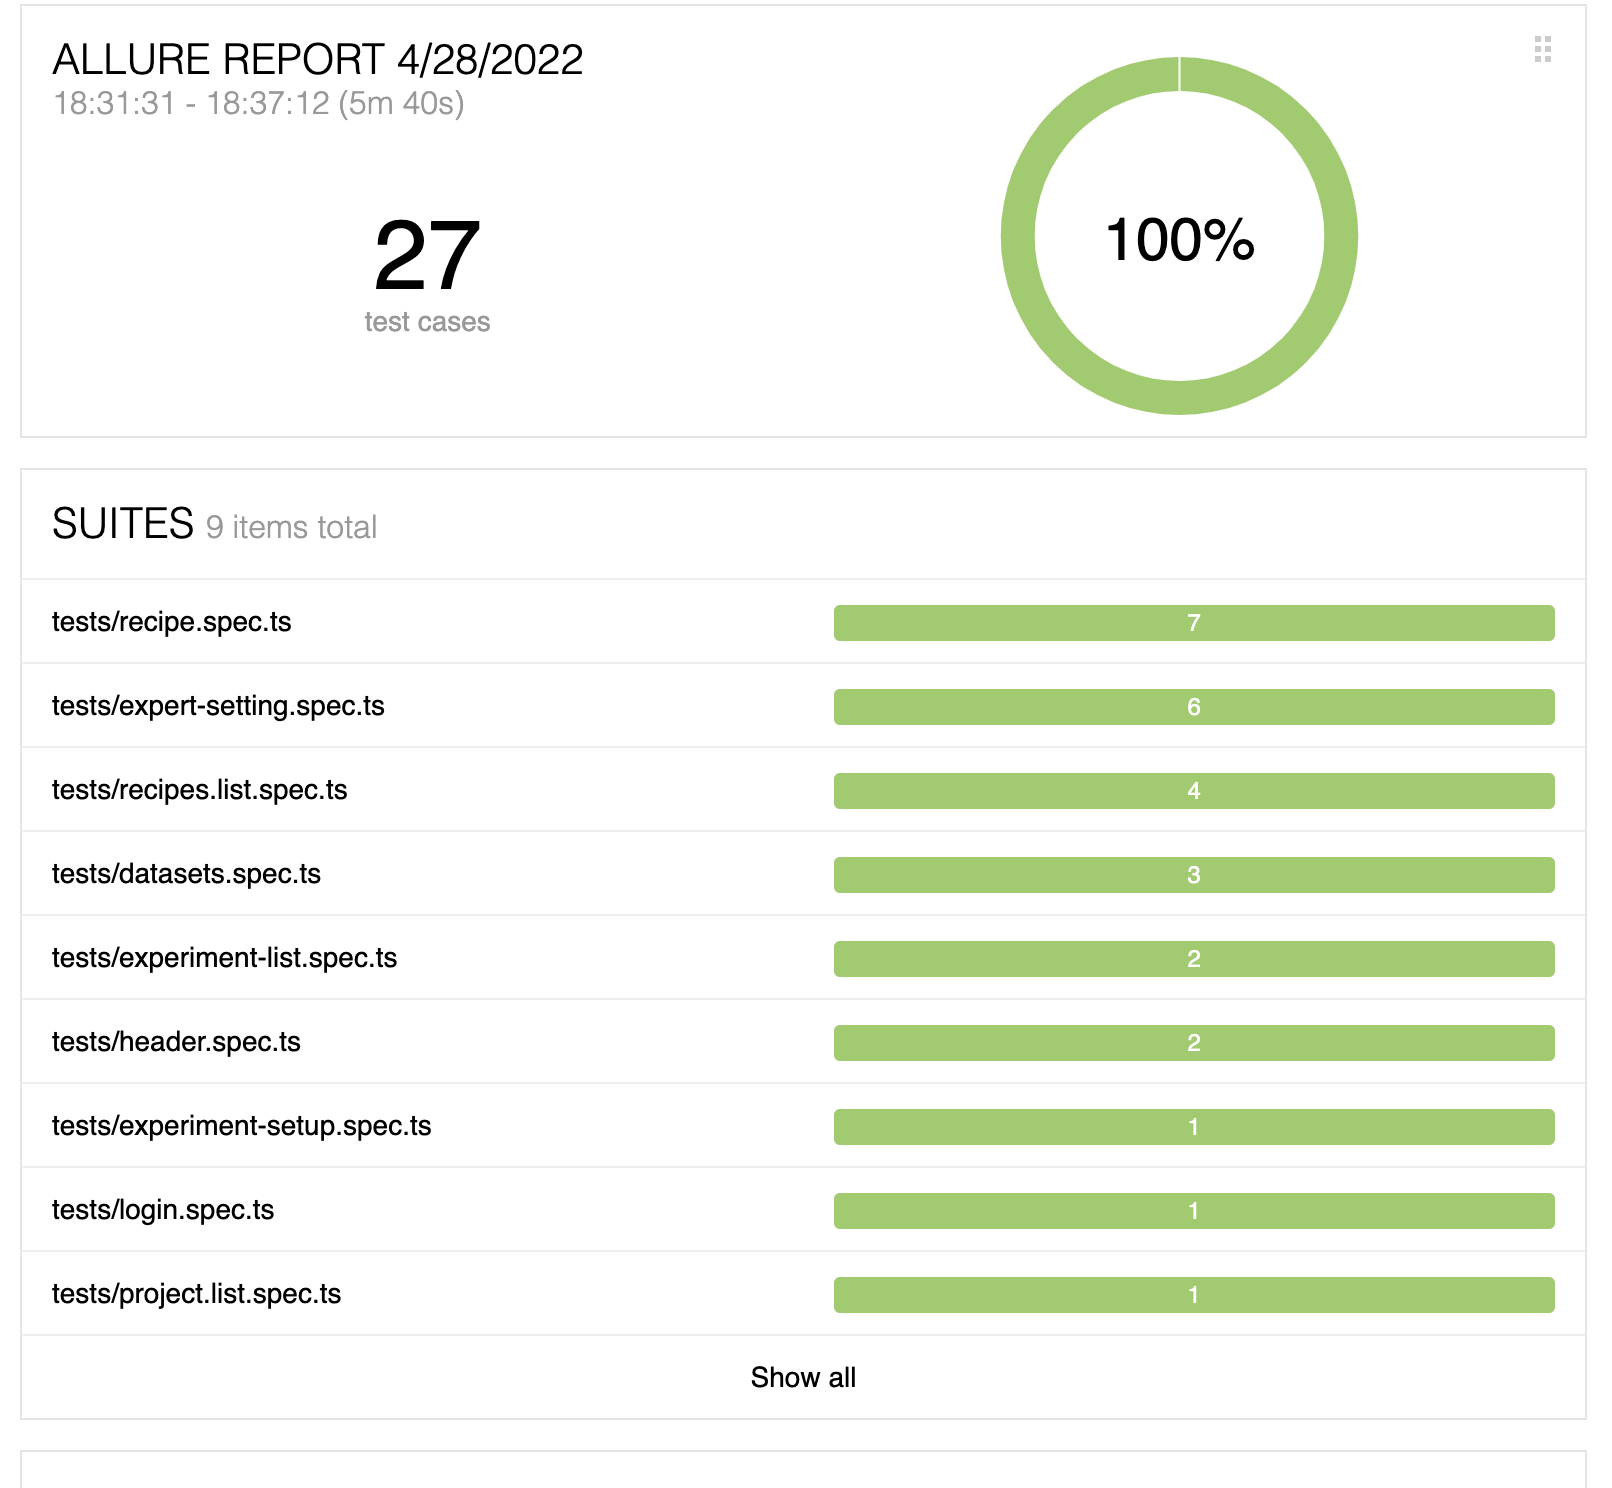
\includegraphics[width=0.8\textwidth]{testReport.png}
\caption{Test Report using Allure for \ac{DAI} GUI Automation Testing by playwright}
\end{figure}

\subsection{ \ac{DAI} Frontend Feature Addition}

I worked on the \ac{DAI} Frontend Feature Addition project at h2oai. This project aimed to add new features to the \ac{DAI} web interface. The goal was to make the web interface more user-friendly and intuitive, allowing users to quickly access and use the features they need.

The first step of the project was to identify potential features that could be added to the \ac{DAI} web interface. We conducted an analysis of user feedback, as well as surveys of existing customers. This enabled us to gain an understanding of which features they would like to see, as well as how they would like to use them.

The second step was to develop the features. We used the H2O Flow framework to create the features, which allowed us to quickly build the features and ensure they were responsive and intuitive. We also implemented automated testing to ensure the features would work correctly, even in extreme scenarios.

The third step was to deploy the features to the \ac{DAI} web interface. We used Docker to deploy the features to a staging environment, where they could be tested and validated by users. After the features had been tested and validated, we deployed them to the production environment.

Finally, we monitored the usage of the newly added features to ensure they were being used correctly and that they were providing the desired benefits. This allowed us to make improvements to the features, as well as identify any issues that may have been overlooked.

Overall, it was a great experience working on the \ac{DAI} Frontend Feature Addition project. I was able to gain a deeper understanding of the web development process, as well as gain valuable experience in developing user-friendly web interfaces.

subsection{Data Science}

I worked on multiple data science projects at h2oai. These projects included the development of machine learning models, as well as the development of data pipelines to process and analyze data. I also worked on the development of data visualization tools to help users visualize and understand the data they were working with.

\subsubsection*{Alternative Credit Scoring (With Graph Analytics)}

Alternative credit scoring is a new approach to assessing the creditworthiness of potential borrowers. It uses the analysis of large amounts of data to develop a more accurate assessment and to provide a more accurate representation of a person's financial standing. This is done by analyzing a range of data sources, such as social media accounts, online behavior, and other sources of public data. Graph analytics is used to create a visualization of the data, which can then be used to assess the borrower's creditworthiness.

Graph analytics uses the connections between different data points to build a visual representation of the data. This visual representation can help to identify patterns and relationships that are not apparent in the data itself. For example, the connections between different accounts, such as a person's social media accounts, bank accounts, and credit cards, can be used to identify patterns in their spending and repayment habits. By aggregating this data, lenders can create a more comprehensive assessment of a borrower's creditworthiness.

Graph analytics can also be used to identify potential risks that may be associated with a borrower. For example, by analyzing the connections between a borrower and their friends, family, and business associates, lenders can identify possible links to fraudulent activity. This type of analysis can be used to identify potential risks that may not have been identified by traditional credit scoring methods.

By combining the analysis of large amounts of data with graph analytics, lenders can create a more accurate and comprehensive assessment of a borrower's creditworthiness. This can help to reduce the risk of fraud, while also providing lenders with a more accurate representation of a borrower's financial standing. This type of analysis can help to improve the accuracy of credit scoring and can provide lenders with a more reliable way to assess the creditworthiness of potential borrowers.

\begin{figure}[H]
\centering
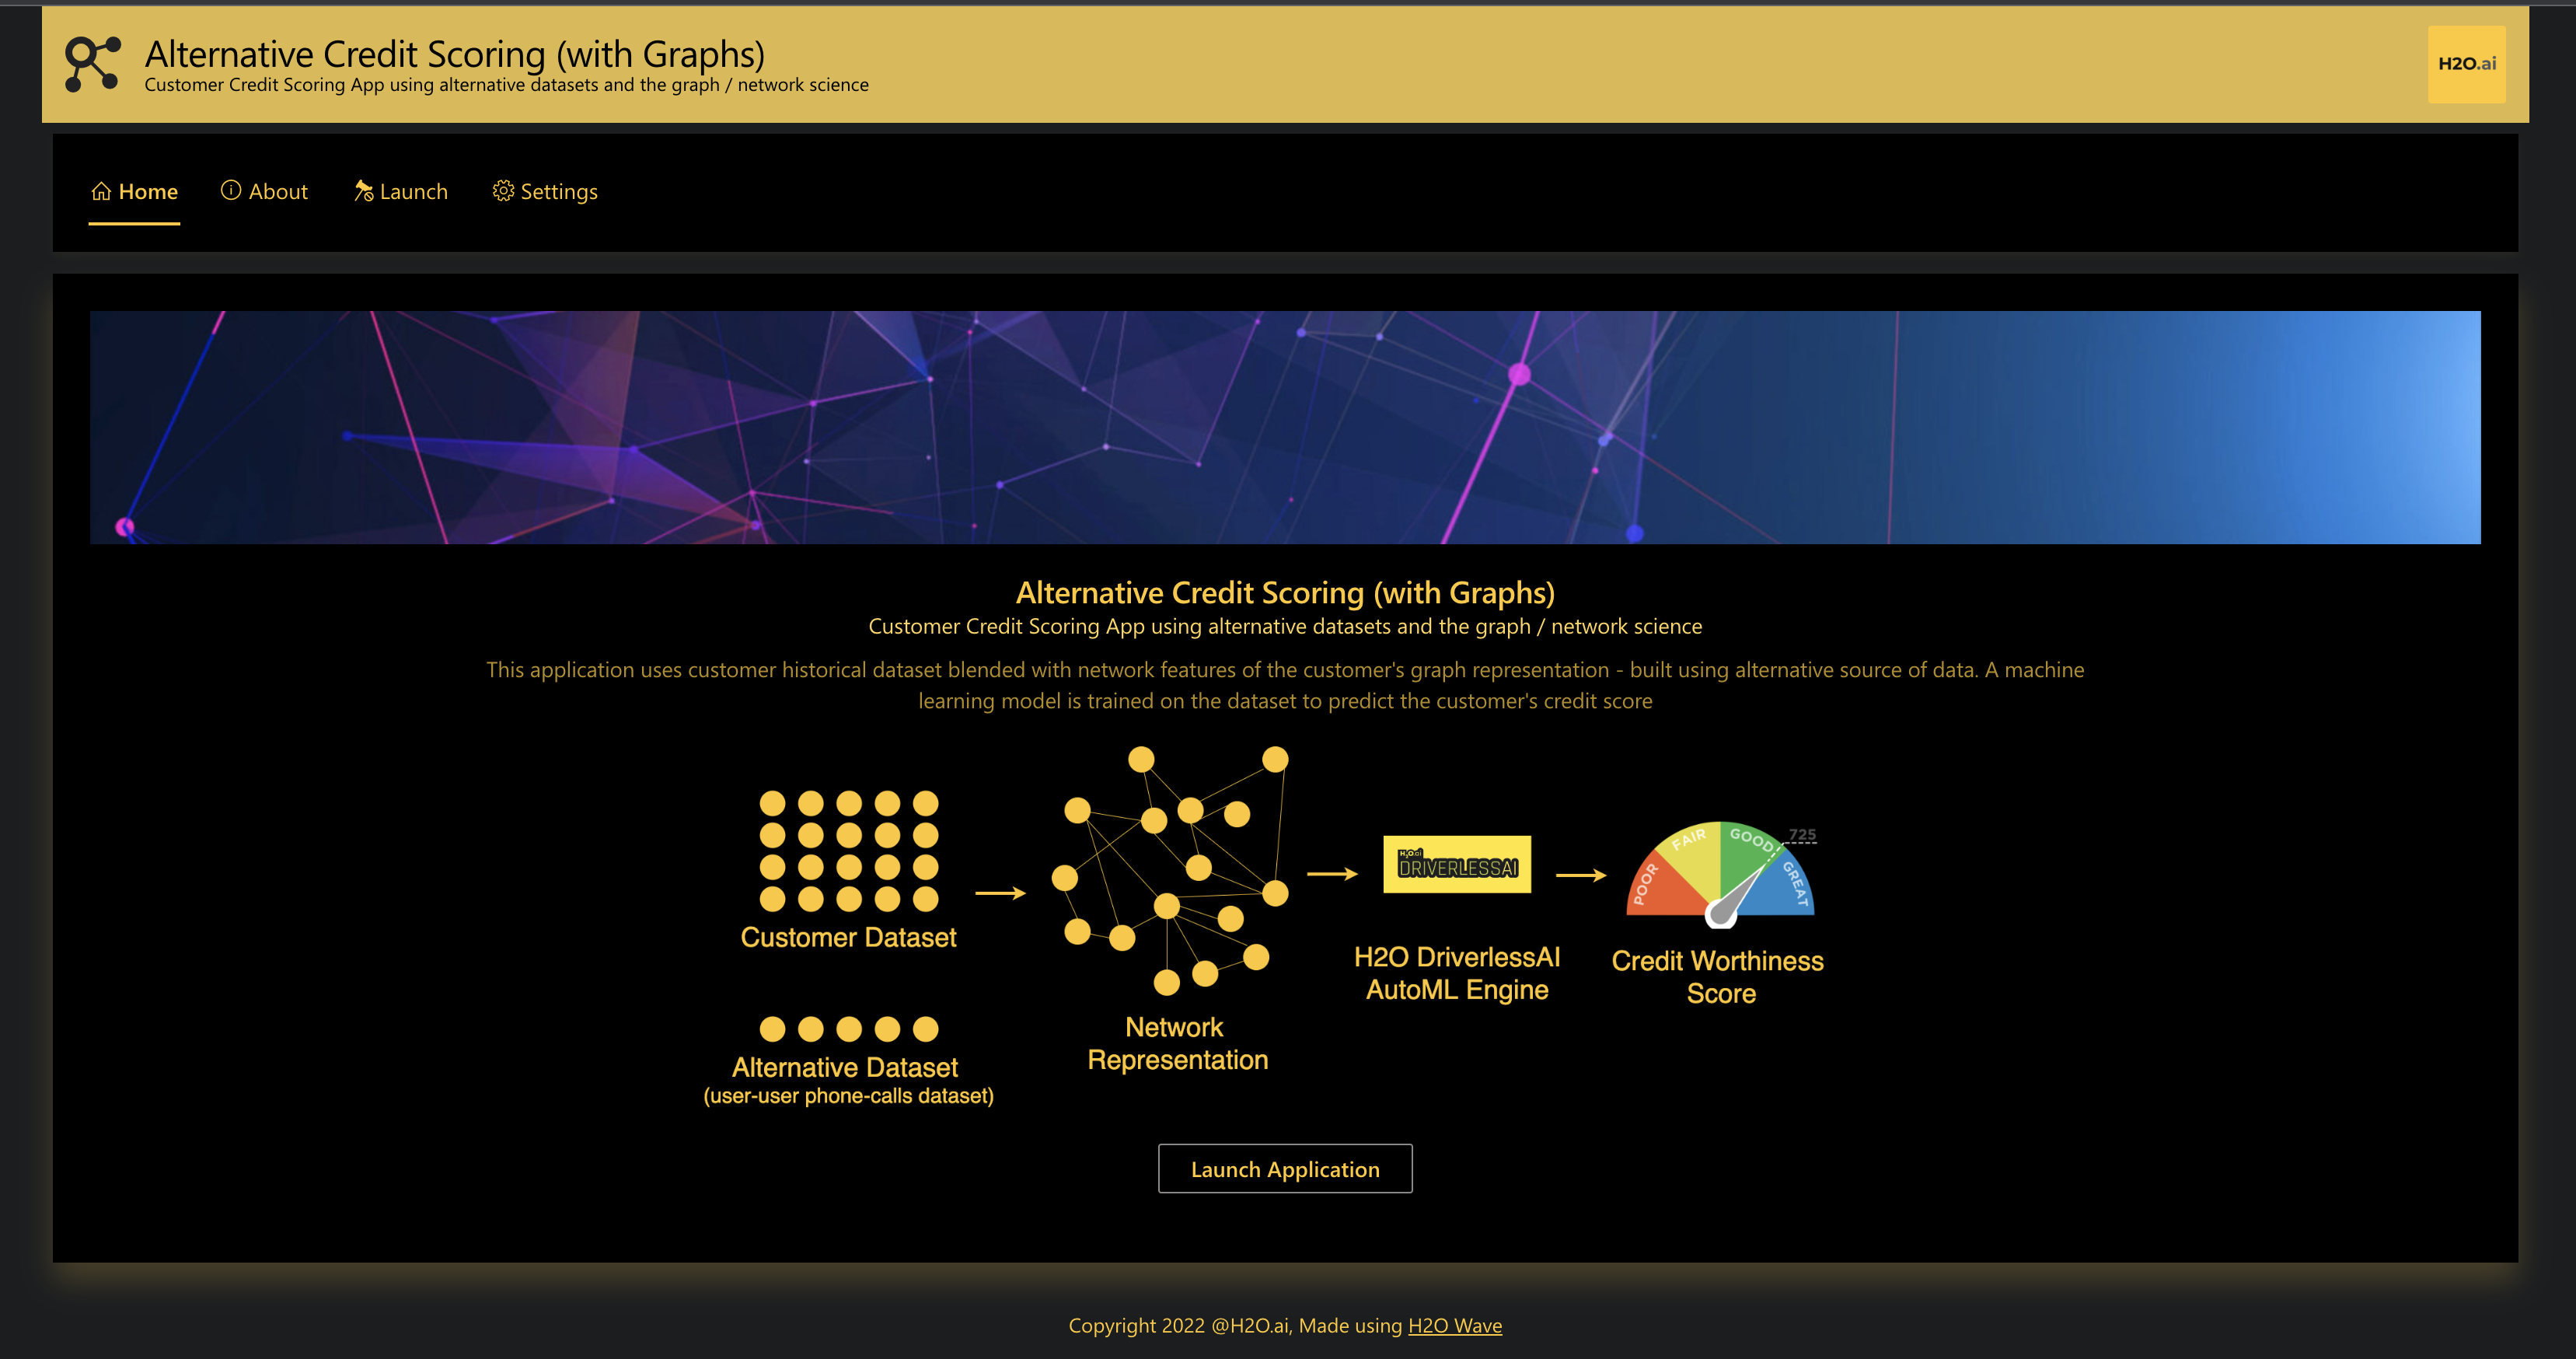
\includegraphics[width=1\textwidth]{a1.png}
\caption{Home Page of ACS App}
\end{figure}

\begin{figure}[H]
\centering
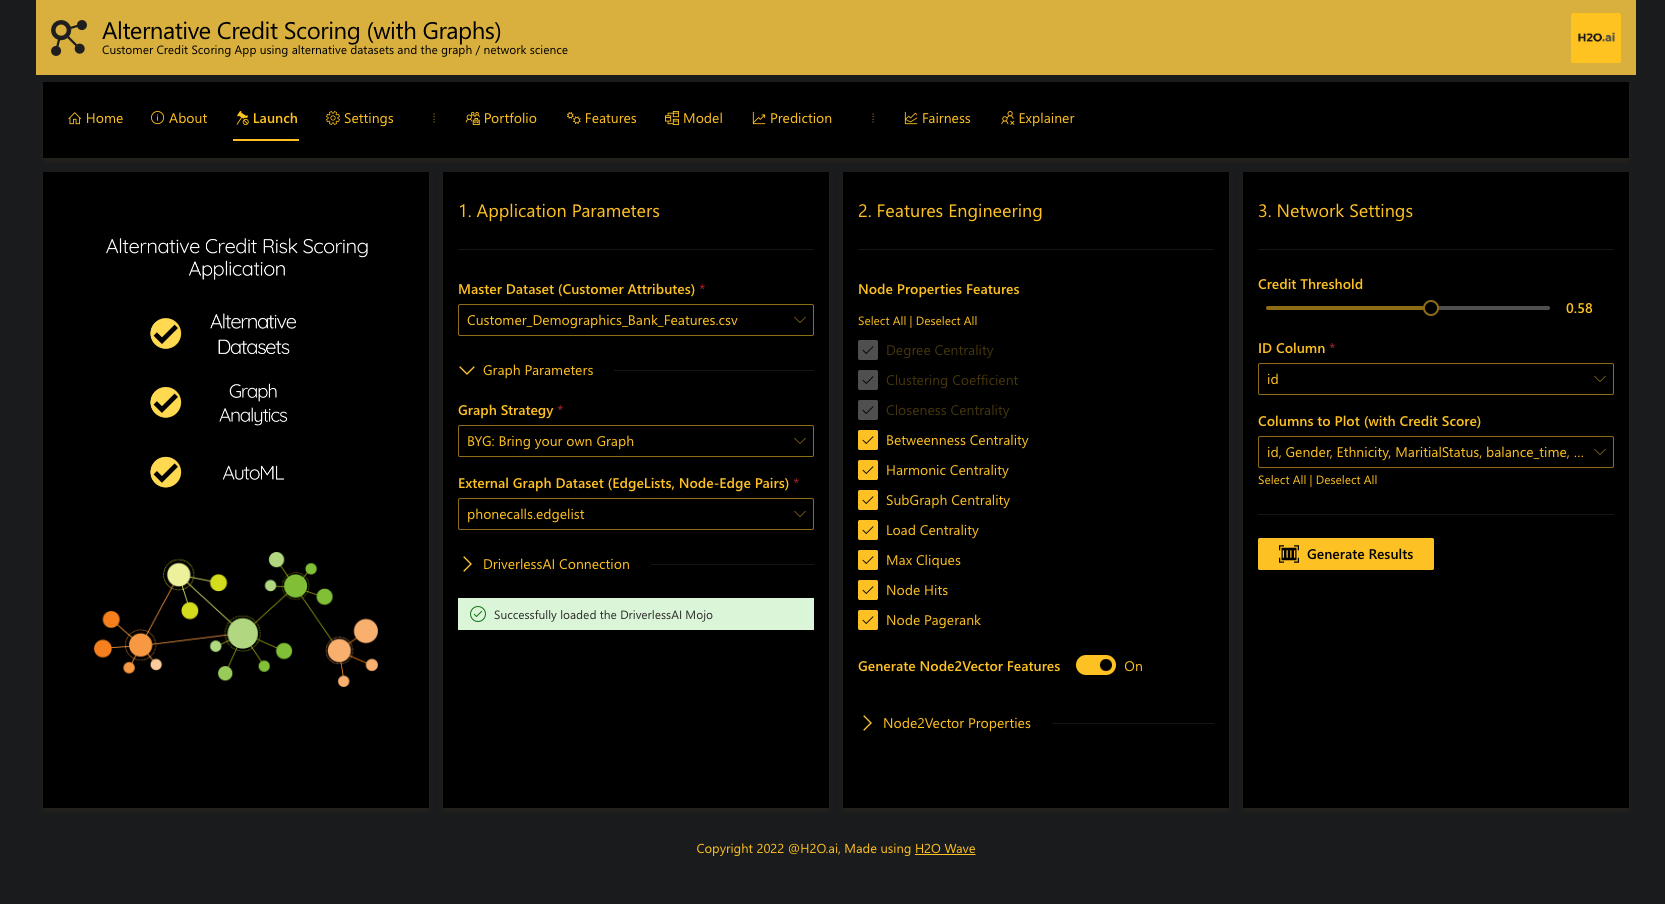
\includegraphics[width=1\textwidth]{a2.png}
\caption{Launch Page of ACS App}
\end{figure}

\begin{figure}[H]
\centering
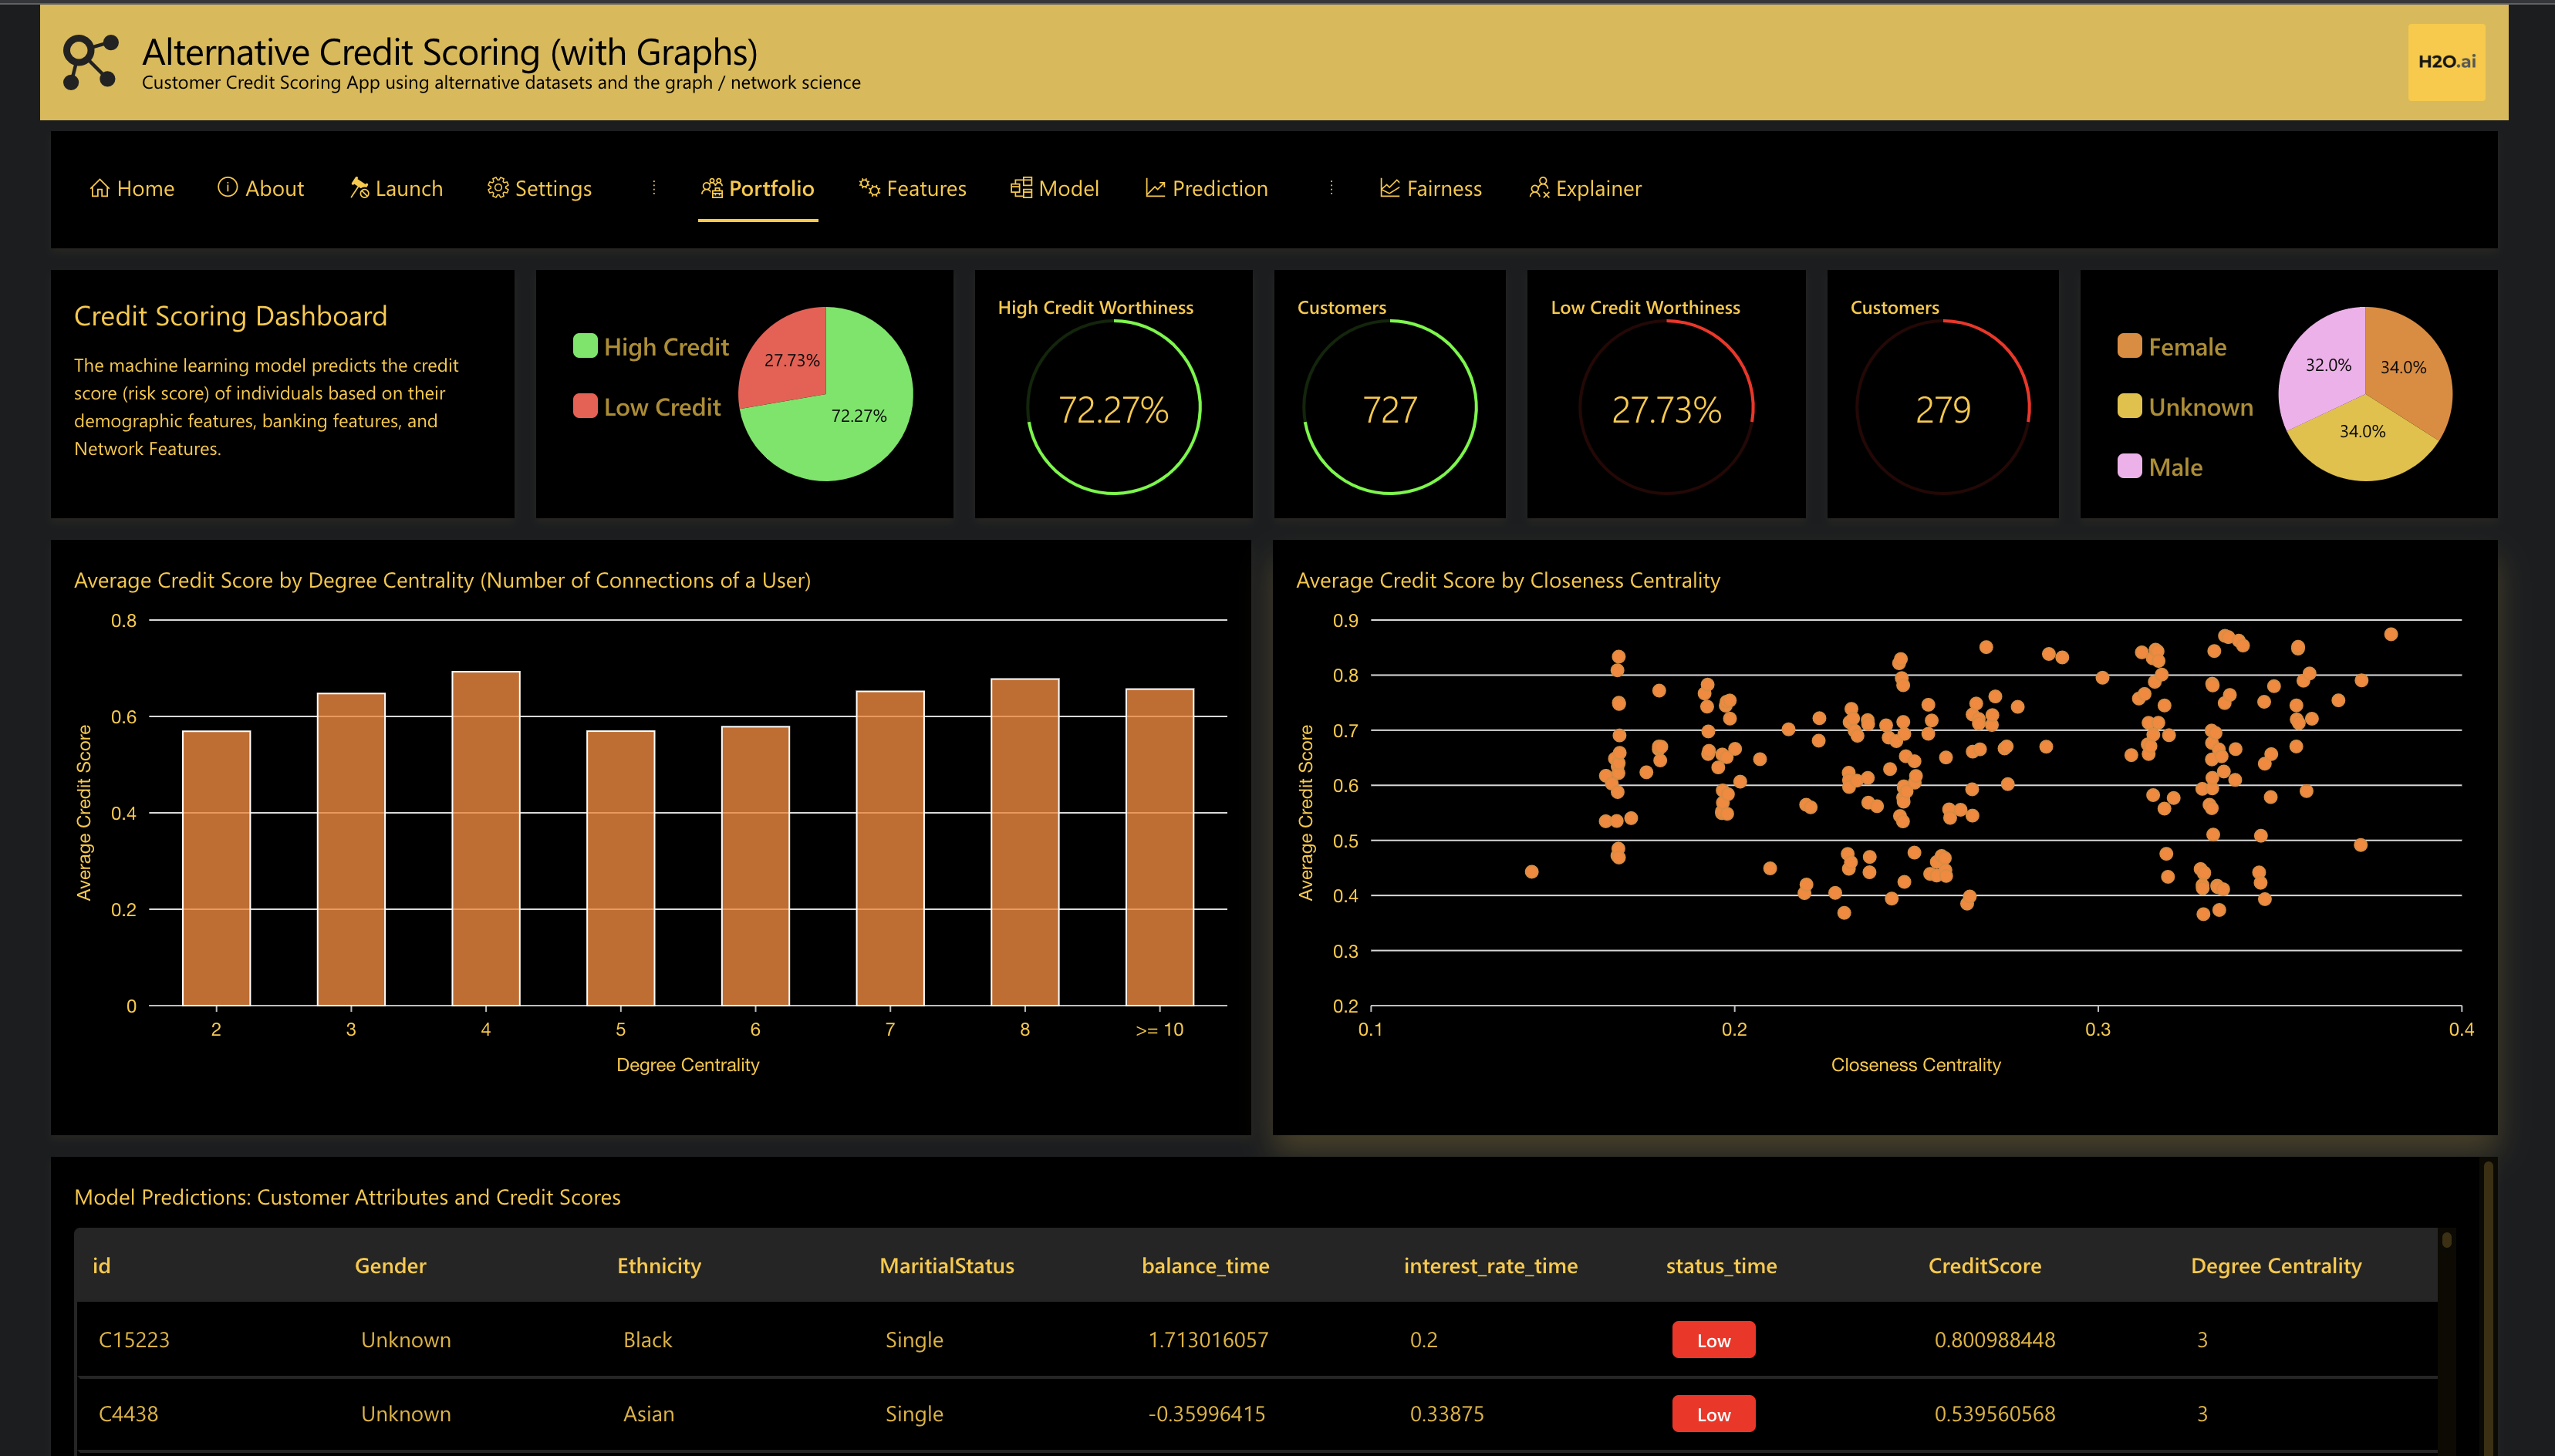
\includegraphics[width=1\textwidth]{a3.png}
\caption{Portfolio of ACS App}
\end{figure}

\begin{figure}[H]
\centering
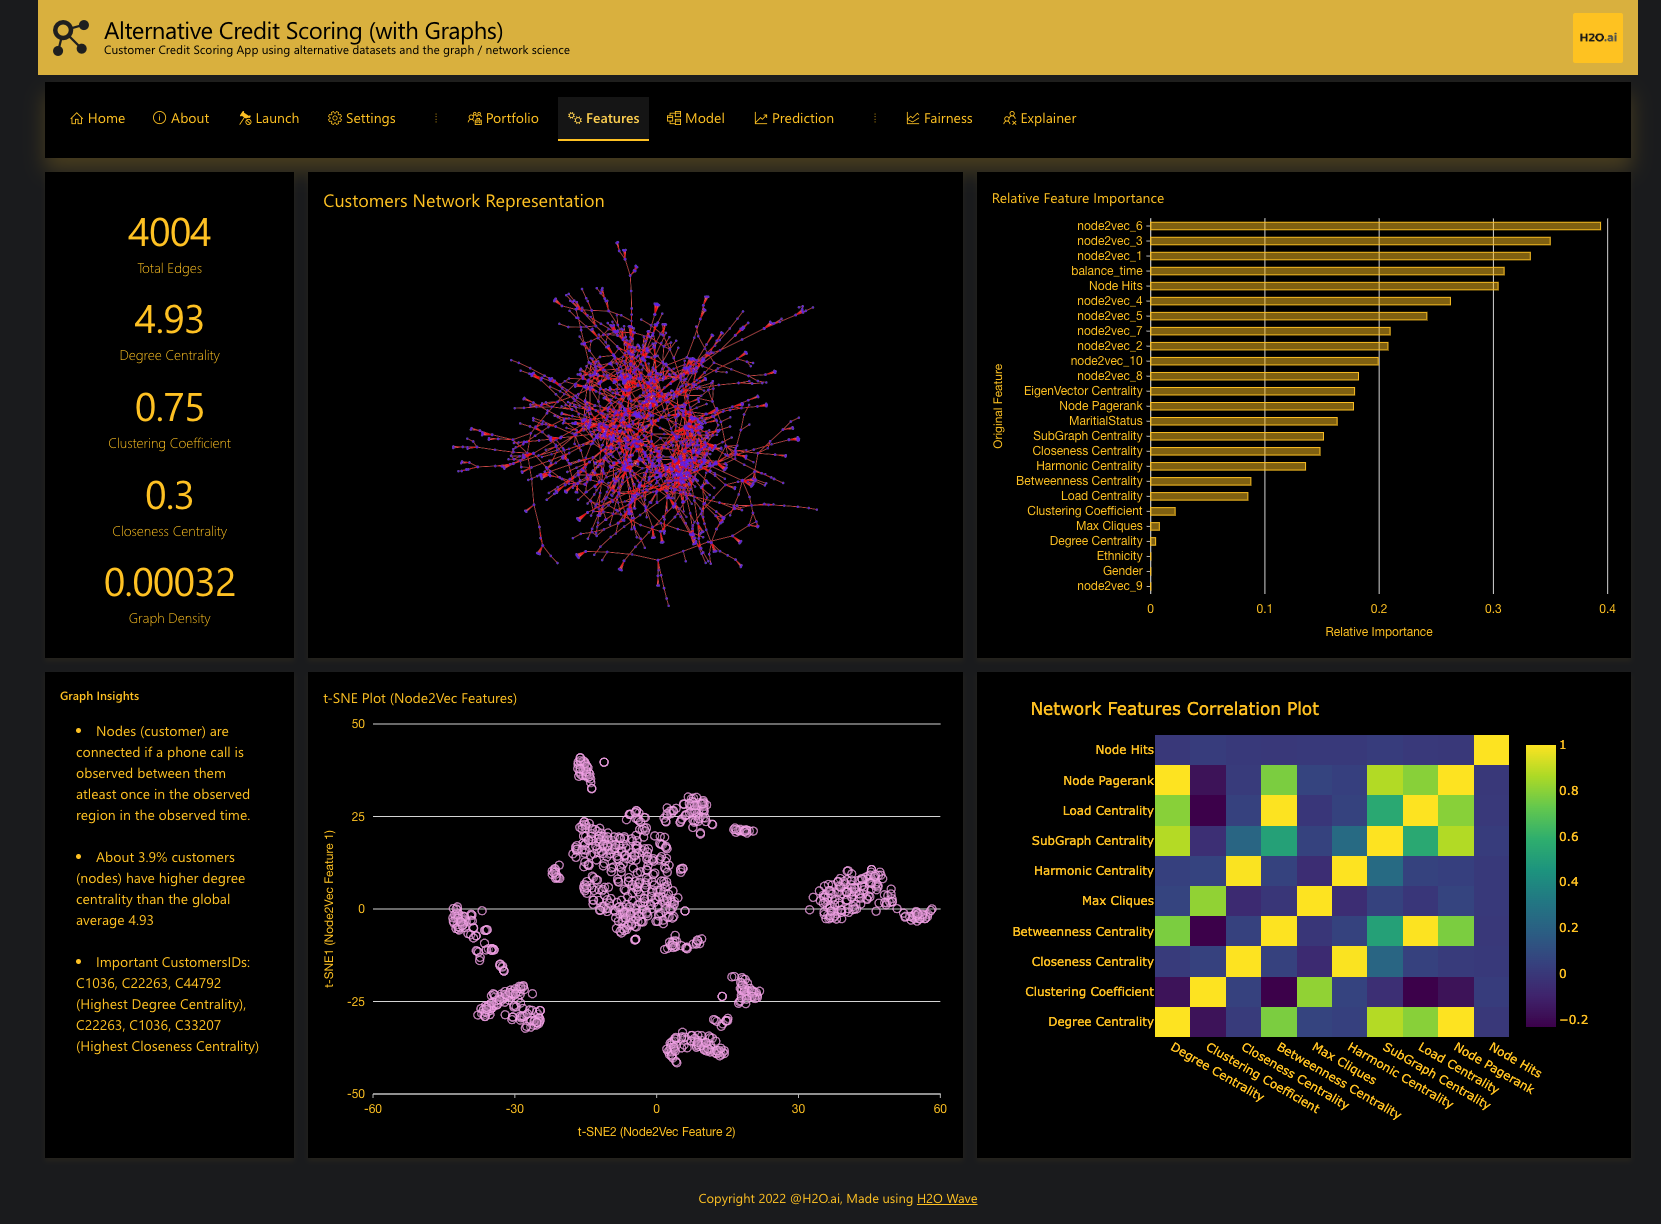
\includegraphics[width=1\textwidth]{a8.png}
\caption{Featues Page of ACS App}
\end{figure}


\begin{figure}[H]
\centering
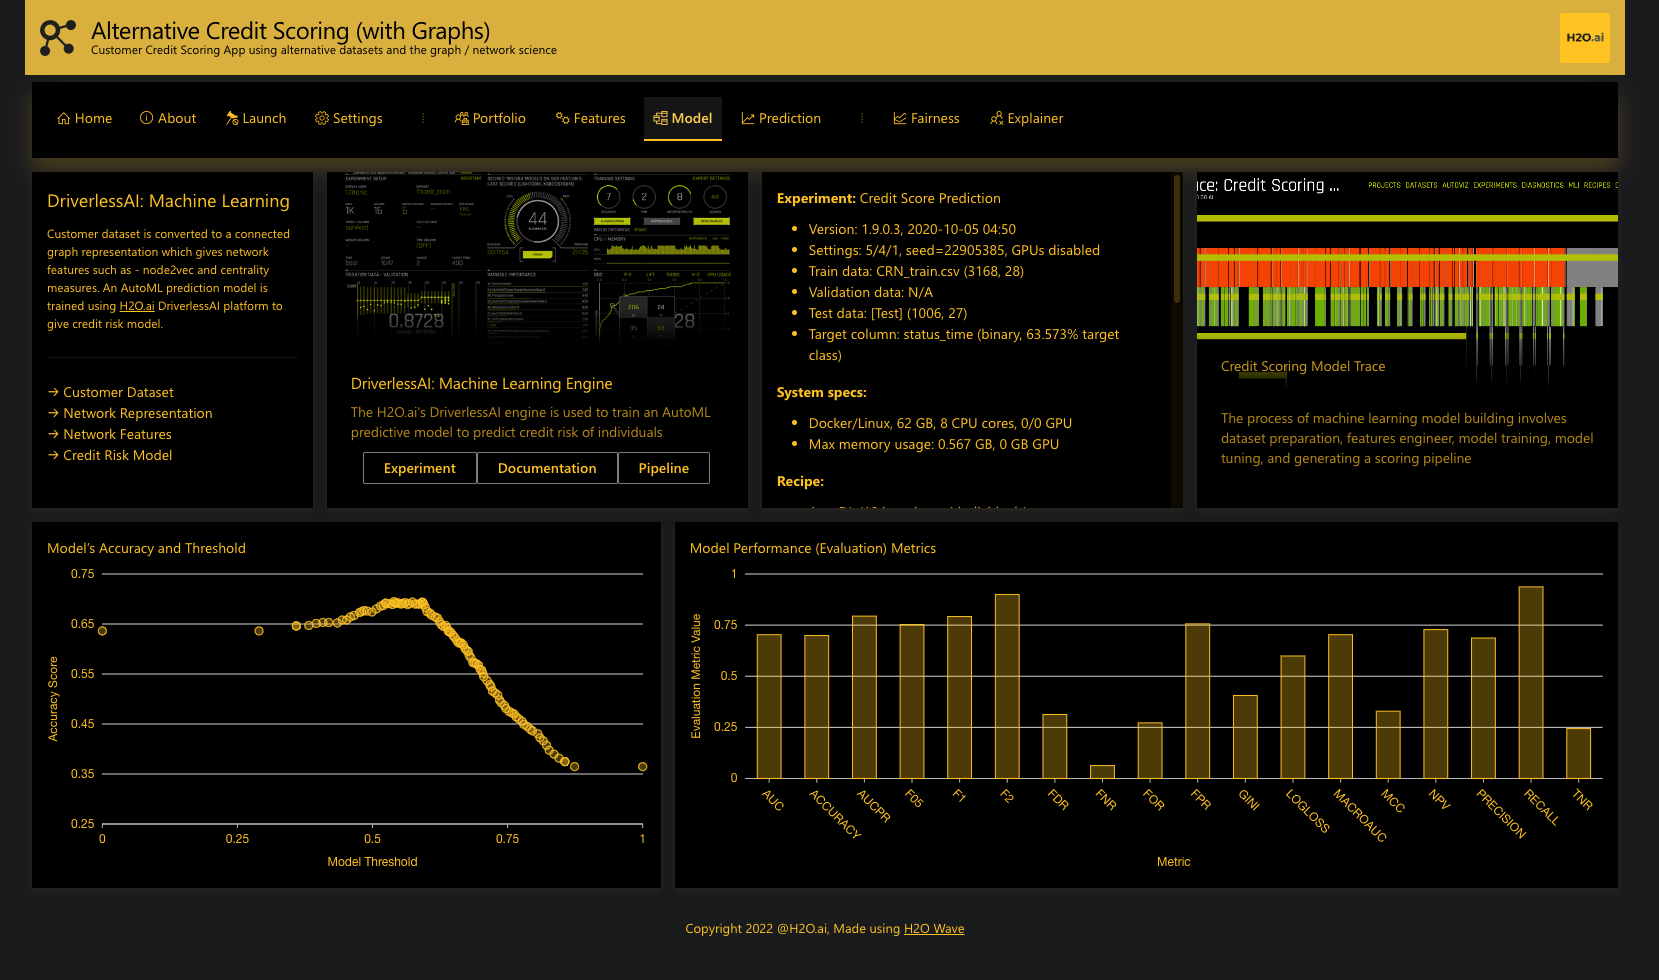
\includegraphics[width=1\textwidth]{a4.png}
\caption{Model Page of ACS App}
\end{figure}

\begin{figure}[H]
\centering
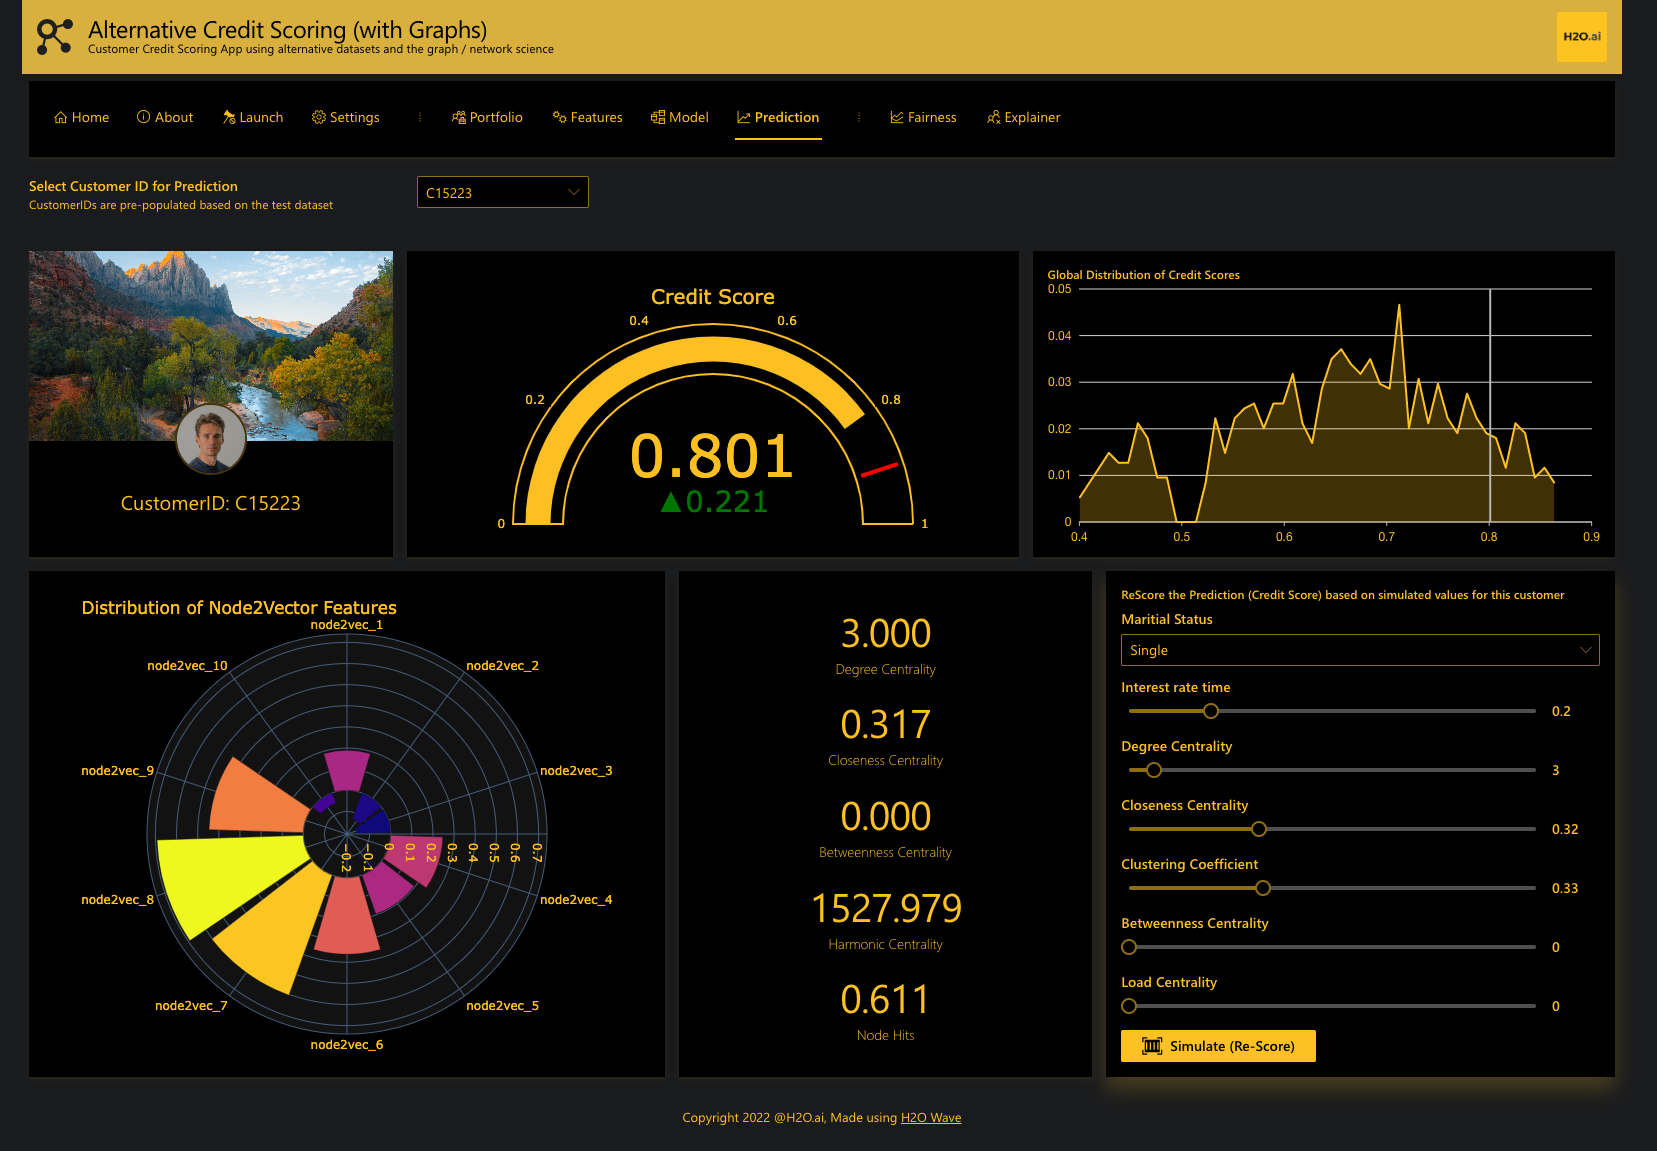
\includegraphics[width=1\textwidth]{a5.png}
\caption{Prediction Page of ACS App}
\end{figure}

\begin{figure}[H]
\centering
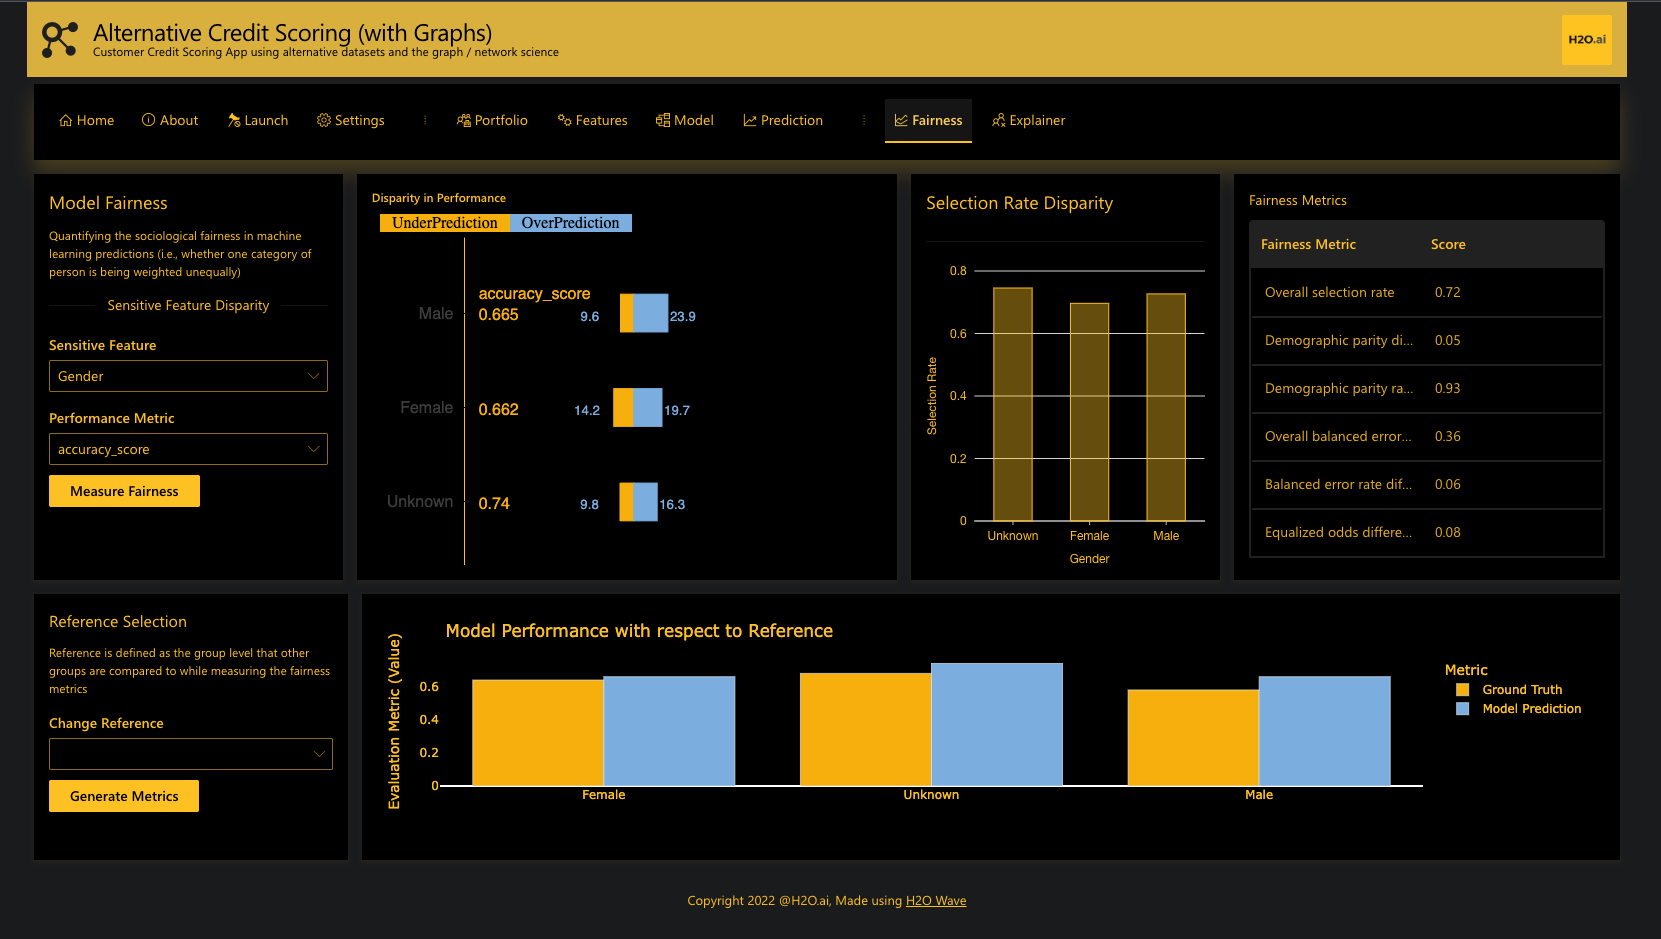
\includegraphics[width=1\textwidth]{a6.png}
\caption{Fairness Page of ACS App}
\end{figure}

\begin{figure}[H]
\centering
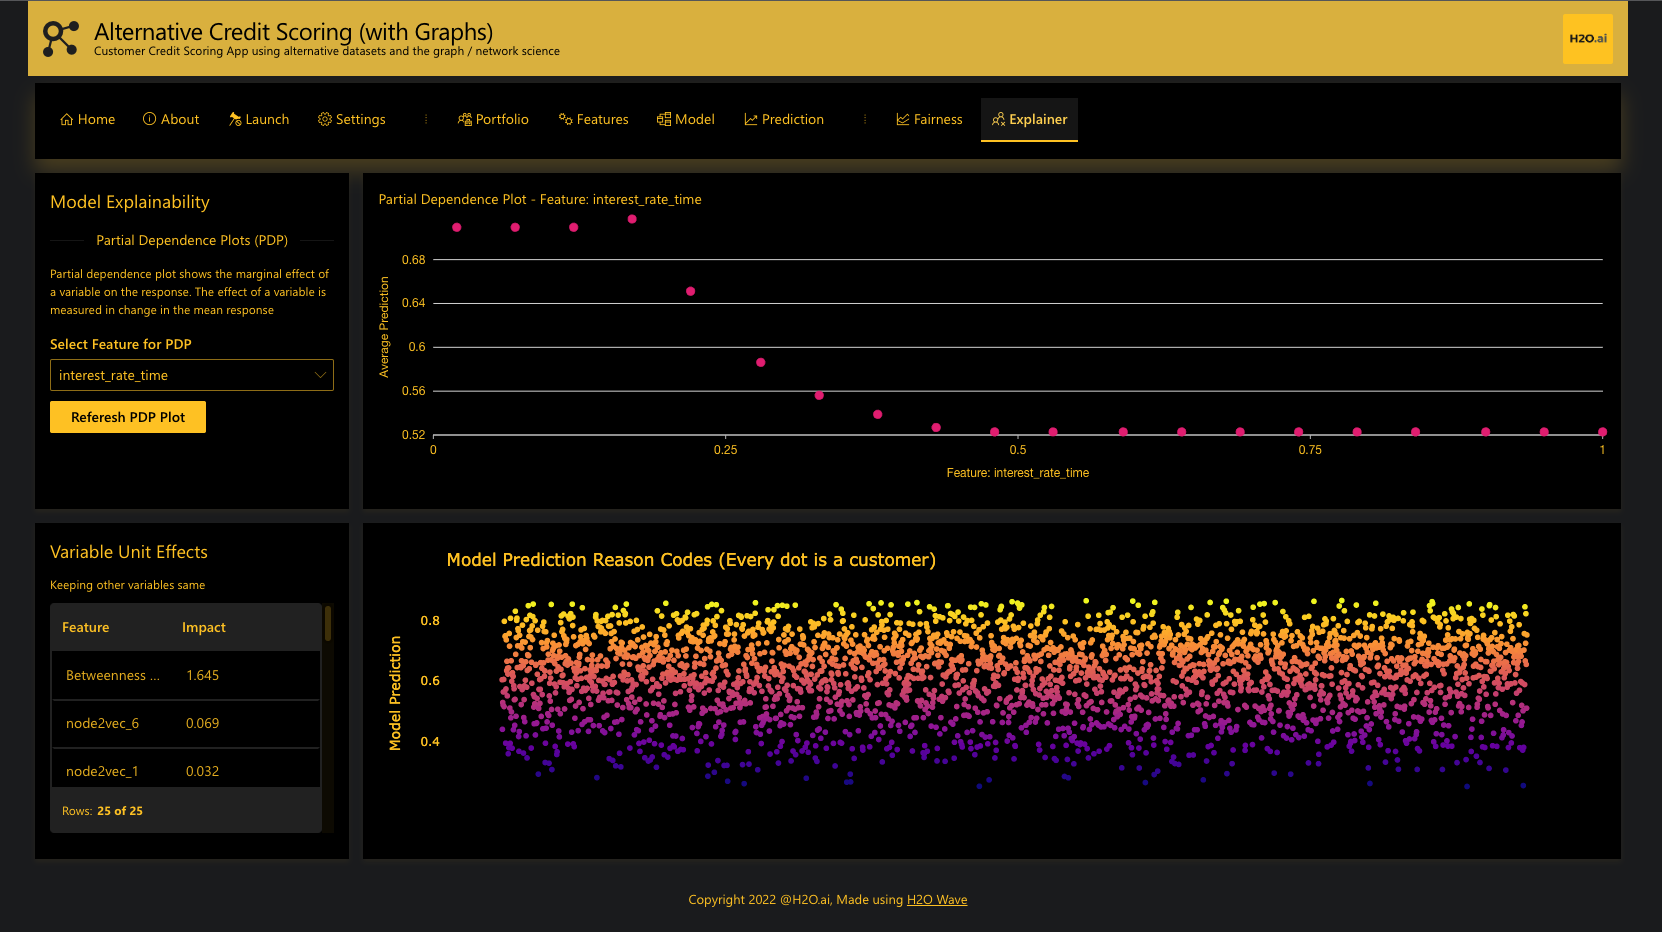
\includegraphics[width=1\textwidth]{a7.png}
\caption{Explainer Page of ACS App}
\end{figure}



\section{Special Training Sessions}

H2O.ai offers special training sessions for Github users to help them understand the powerful machine learning and analytics platform. The sessions cover topics such as setting up a Github account, configuring repositories, and using the Git command line. The sessions also provide an overview of basic concepts and best practices in using the platform. Additionally, hands-on exercises are included to get participants up and running quickly with Github. These sessions are designed to help users become proficient with the platform and enable them to take advantage of its features to create and share their own projects.

\section{Non-Technical Experience}


At H2O.ai I have had the opportunity to gain valuable non-technical experience and skills that can be used in the workplace. The most valuable of these are: 

1. Communication: Working with a diverse team of data scientists, engineers, and product managers has taught me how to effectively communicate with others. I have learned how to break down complex ideas into more digestible chunks, which is key to conveying important information to those who may not be as familiar with technical concepts. Additionally, I have learned how to effectively listen to my colleagues and take into account multiple perspectives on a given issue.

2. Problem Solving: Working at H2O.ai has given me the opportunity to work through challenging problems. This has taught me how to break down a problem into manageable pieces and think critically about possible solutions. As a team, we have collaborated to come up with innovative solutions to complex problems.

3. Teamwork: Working in a collaborative environment has taught me the importance of teamwork. I have learned how to work well with others in order to efficiently complete tasks and meet deadlines. I have also gained a better understanding of how to effectively delegate tasks and roles in order to ensure that everyone is contributing in the most effective way.

4. Leadership: Working in a leadership role at H2O.ai has given me the opportunity to develop my leadership skills. This has included developing strategies and plans for projects, managing resources, and motivating my team to reach our goals.

Overall, my experience at H2O.ai has given me the opportunity to gain valuable non-technical experience and skills that can be applied in any workplace. These skills will help me to become a better communicator, problem solver, team member, and leader.


\chapter{Conclusions}

\section{Summary of Training Experience}

H2O.ai is a great place to work with a unique culture that values collaboration, creative problem solving, and an entrepreneurial spirit. Everyone is focused on making a positive impact and making data science easier for everyone. I've been able to work alongside some of the brightest minds in the industry and collaborate with them on projects to develop innovative solutions.

The company has a strong focus on customer success, which is evident in the way they provide technical and non-technical support to all of their customers. They have a great customer success team that is always available to answer questions and provide guidance.

The team at H2O.ai is also incredibly welcoming. Everyone I've interacted with has been friendly and eager to help. From the leadership team to the engineers and data scientists, everyone is focused on making sure customers have the best experience possible.

The company also has an amazing culture of learning and development. Everyone is encouraged to attend conferences, take courses, and participate in hackathons. This helps to keep everyone up to date on the latest technologies and innovations in the field.

Overall, my experience at H2O.ai has been incredibly positive and I would highly recommend it to anyone looking for a company that values collaboration, creative problem


\section{Training Program at H2o.ai}


H2o.ai's training program is well structured, with a focus on hands-on learning and providing an immersive experience. The program is designed to help participants gain knowledge and build skills in data science and AI. Participants are provided with resources and guidance throughout the program, and they are encouraged to take ownership of their learning. Mentors are assigned to each participant to provide individualized guidance and feedback. The mentors provide a personalized learning experience and help ensure each participant is able to maximize their learning. The program also includes weekly meetings, feedback sessions, and resources to ensure that participants are able to stay on track and gain the most out of their training experience.

\section{Suggessions for Traning Establishment}
I suggest H2O.AI focus on introducing new features and tools to make the user experience more efficient. This could include developing a more user-friendly interface for applications, introducing automation to simplify data exploration and analysis, and providing better documentation and tutorials for those new to the platform. Additionally, H2O.AI could look into introducing AI-based algorithms and methods to improve the accuracy and speed of data analysis. Finally, I suggest H2O.AI works on improving the scalability of the platform, allowing businesses to take advantage of large datasets to gain insights quickly and efficiently.


\printbibliography
\addcontentsline{toc}{chapter}{References}

\end{document}